\chapter{Theoretical Framework}
This chapter allows to know the basic concepts required for understanding the development under the proposed project. The field of biosensors is comprised of elementary concepts of electronics, chemistry, materials science, and biology. The functional printed electronics and inkjet printers require theoretical clarifications according to the project to be developed. Fundamental principles of biosensors, functional printed electronics techniques, ink jet printing, the materials to be used and the characterizations to be performed will be analyzed.

\section{Sensors, transducers and biosensors}
A \textbf{sensor} is a device capable of transforming physical or chemical quantities, called instrumentation variables, into electrical quantities through a transducer. These devices can be characterized by different properties such as the measurement range, precision, linearity, repeatability, among others. The instrumentation variables can be magnitudes such as temperature, pressure, humidity, pH, light intensity, distance, acceleration, inclination, displacement, force, torsion, movement, etc. In a broader meaning, it is the expansion of the senses to acquire a knowledge of physical and chemical quantities that, due to their nature or size, cannot be directly perceived by the senses \cite{PallasAreny}.

A \textbf{transducer} transforms the variation in sensor property into an information output detectable by an electronic system. It may or may not have a signal conditioner within the same device, typically with one of the outputs for industrial use: voltage output (V) or standard current output (4 to 20 mA)(Figure ~\ref{fig:Figura_concepto_sensor}).

\begin{figure}[H]
  \centering
    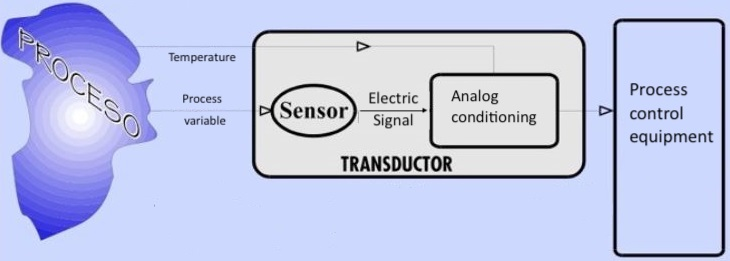
\includegraphics[width=0.8\textwidth]{Figures/Figura_concepto_sensor}
  \caption{Sensor and transducer diagram. Figure taken and traduced from \cite{Hector1}.}
  \label{fig:Figura_concepto_sensor}
\end{figure}

A \textbf{biosensor} can be defined as a device that recognizes a certain analyte by means of a \textbf{bioreceptor} coupled to a \textbf{physicochemical transducer} that converts the biological signal into an electrical signal (Figure ~\ref{fig:Figura_Biosensor}), this signal being proportional to the group of compounds to be determined qualitatively or quantitatively. An analyte is the component of analytical interest of a sample. In the case of biosensors, a protein molecule, a toxin, a peptide, a vitamin or a metal ion are examples. The bioreceptor can be a simple or complex biomolecule (enzymes, antibodies, nucleic acid chains), or based on cells (tissues, organisms) and can be taken from nature or synthesized in a laboratory. The transducer can be of the resonant, optical, thermal, FET (\textit{Field-Effect Transistor}), surface acoustic wave, piezoelectric, or electrochemical type. Within the latter, the conductivity, amperometric, potentiometric and impedometric types can be distinguished \cite{Eggins}.

\begin{figure}[H]
  \centering
    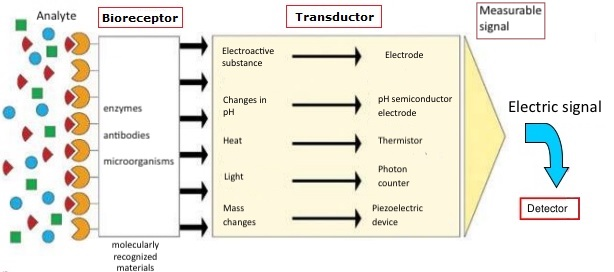
\includegraphics[width=0.8\textwidth]{Figures/Figura_Biosensor}
  \caption{Biosensor diagram: bioreceptor, transducer and electronic signal conditioner. Figure taken and traduced from \cite{Lili1}.}
  \label{fig:Figura_Biosensor}
\end{figure}

Electrochemical transducers are the most widely used in the development of enzyme biosensors. This is because they have a number of advantages, such as:

$\bullet$ Electrochemical measurements can be performed in small volumes, even on the order of nanoliters, with relative ease. This makes such devices especially suitable for monitoring in $``$\textit{in vivo}$"$.

$\bullet$ The electrical signal obtained is the direct transduction of the chemical reaction rate.

$\bullet$ The detection limits that are obtained, normally between 10\textsuperscript{-9} and 10\textsuperscript{-6} mol$\cdot$l\textsuperscript{-1}, are sufficient and adequate for the detection of numerous analytes of interest.

$\bullet$ The relative simplicity and low cost of electrochemical instrumentation allow for easy availability of these devices.

Undoubtedly, in the context of electrochemical biosensors, the most promising in terms of sensitivity, selectivity, size, portability and a minimum volume of sample (analyte) required are the amperometric biosensors, object of study of the present integrating final project. These sensors monitor pharadaic currents (direct transfer of electrons via an oxidation reaction in one electrode and a reduction reaction in the other) between the biological system and a typical electrochemical cell made up of three electrodes: a working electrode \emph{(WE)}, one reference \emph{(RE)} and a counter electrode \emph{(CE)} (Figure ~\ref{fig:Figura_Definicion_Electrodo}). The electrochemical reaction occurs in the \emph{WE}, for which a variable potential is applied with respect to the fixed potential \emph{(RE)} electrode. The current resulting from the chemical reaction circulates between the \emph{WE} and the \emph{CE}. The variation of applied potential and the current measurement are controlled by means of a potentiostat.

\begin{figure}[H]
  \centering
    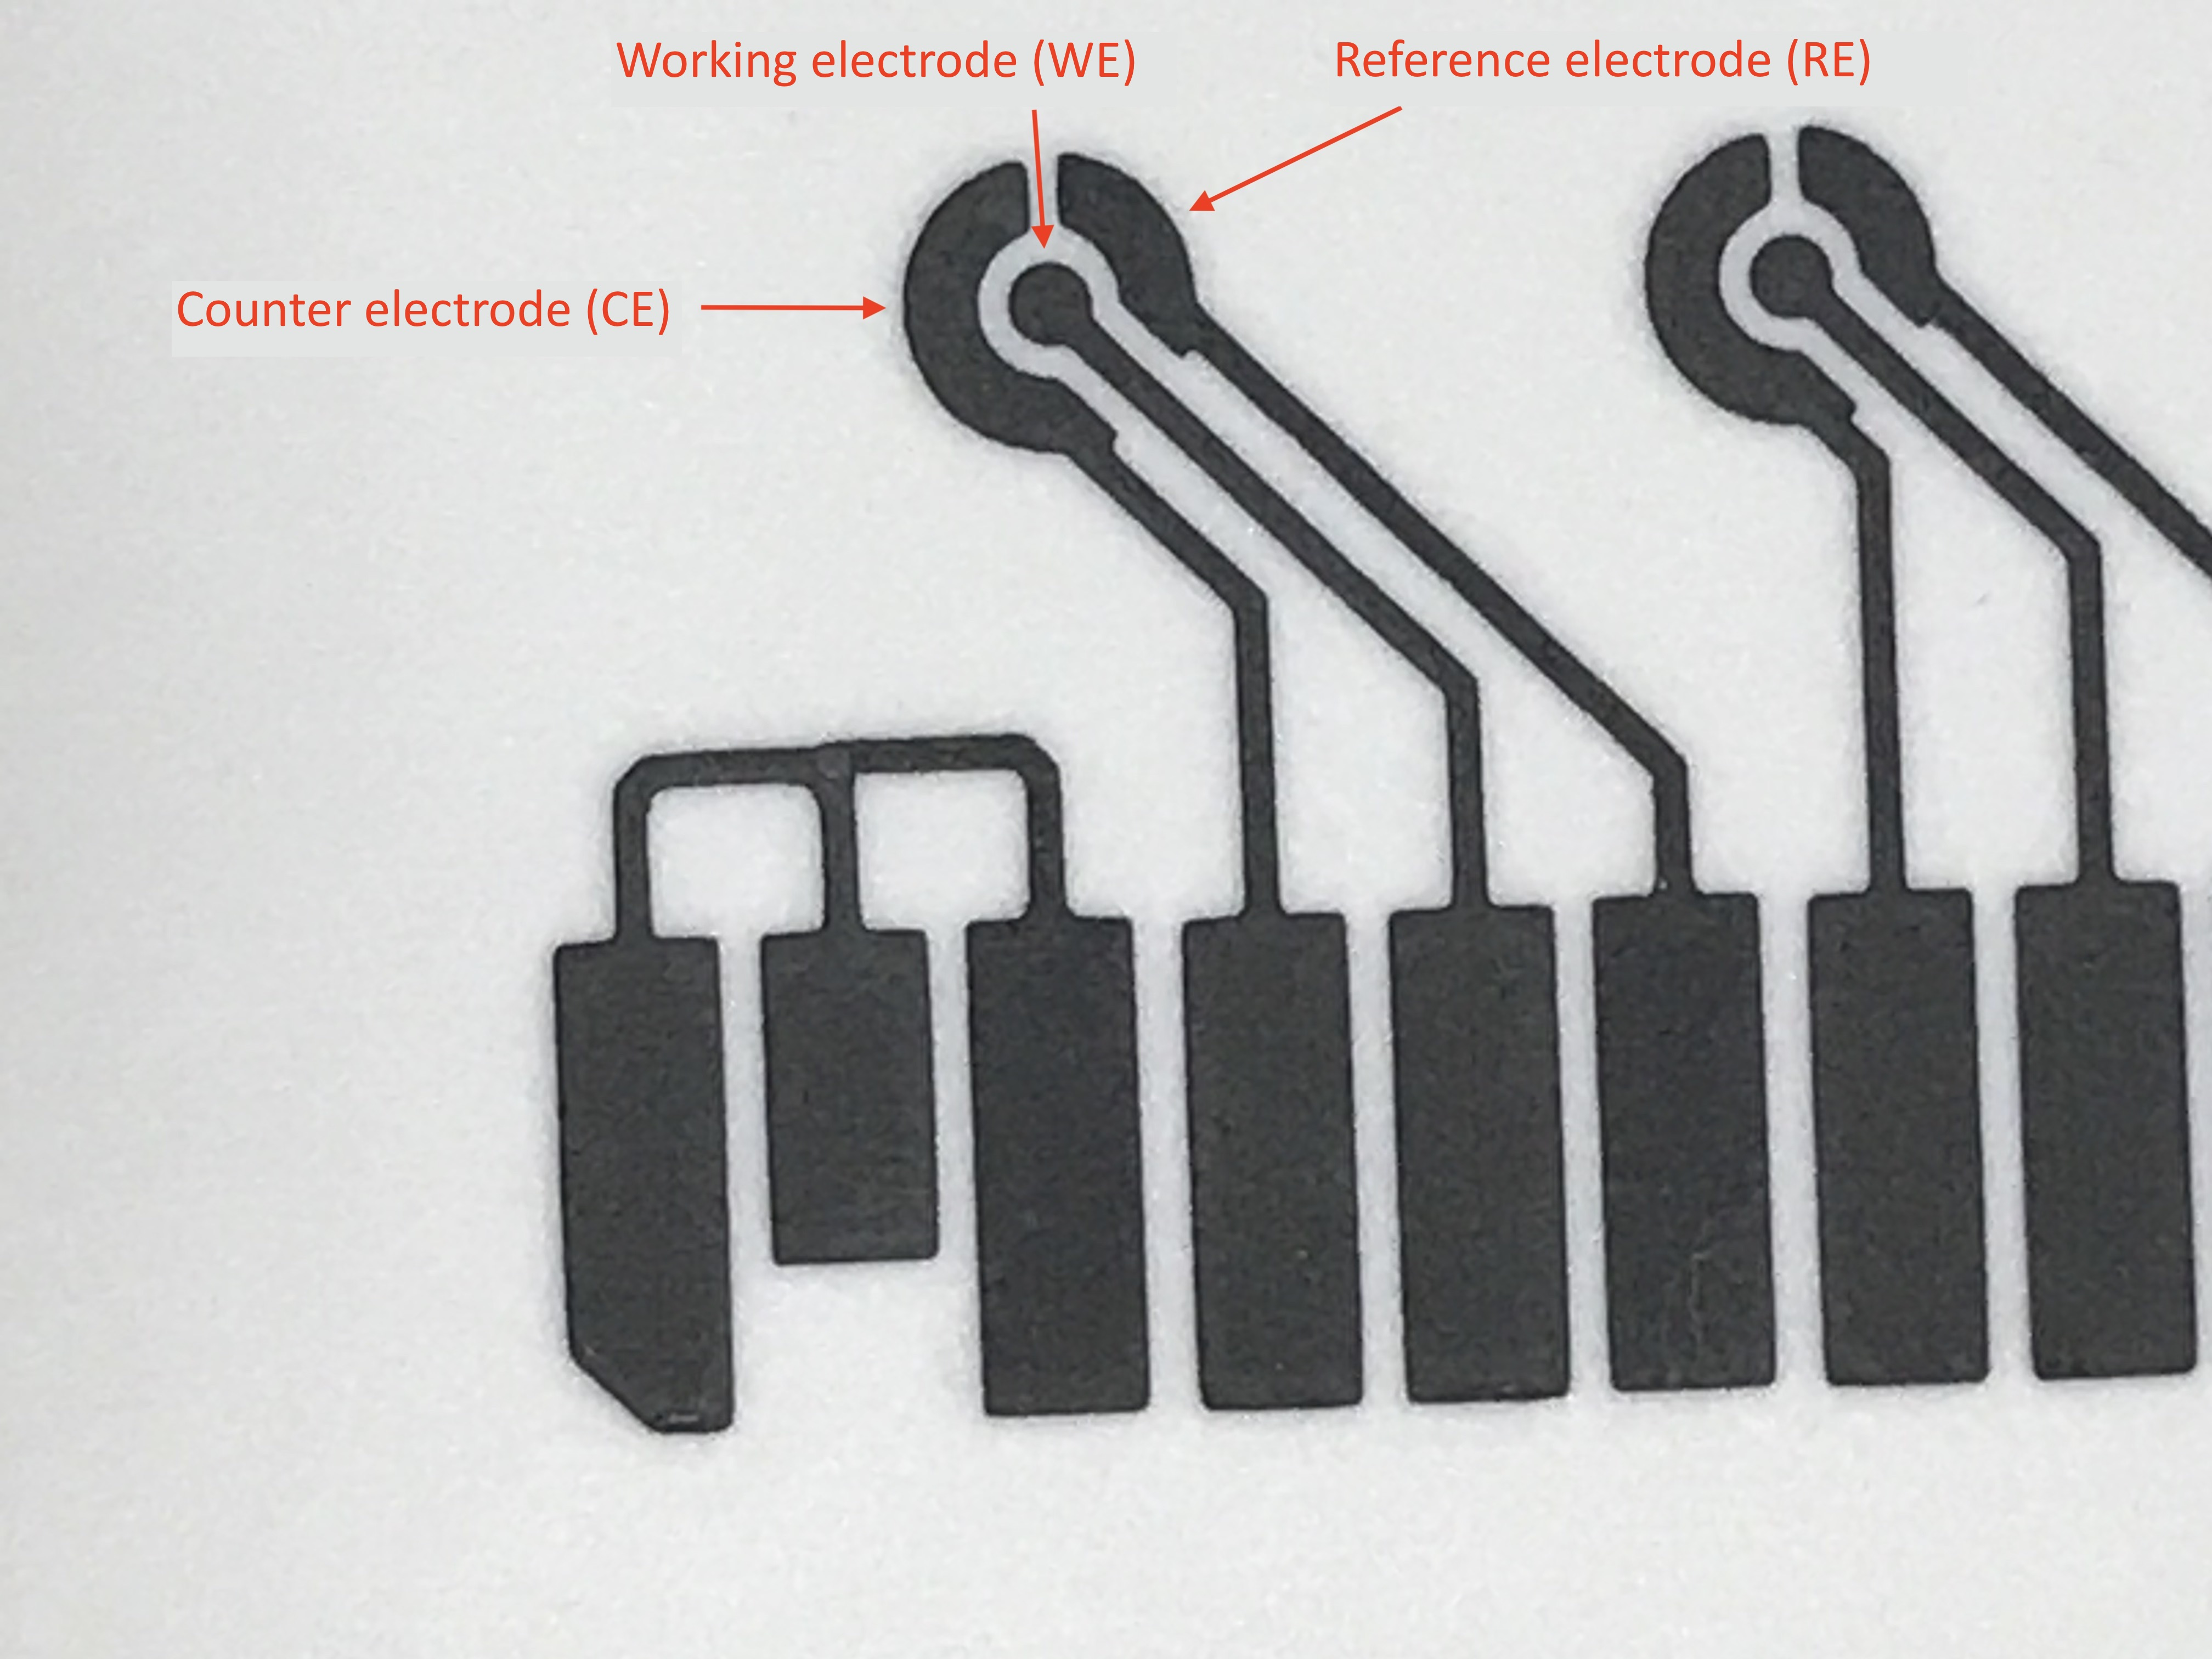
\includegraphics[width=0.5\textwidth]{Figures/Figura_Definicion_Electrodo}
  \caption{Electrochemical Biosensor.}
  \label{fig:Figura_Definicion_Electrodo}
\end{figure}

A potentiostat (Figure ~\ref{fig:Figura_potenciostato}) is an electronic device used to control a three-electrode cell and to perform most electroanalytical experiments. Its function is to apply a variable potential on the \emph{WE} with respect to the fixed potential applied on the \emph{RE} and to measure the resulting current that circulates between the \emph{WE} (where the electrochemical reaction occurs) and the \emph{CE}.

\begin{figure}[H]
  \centering
    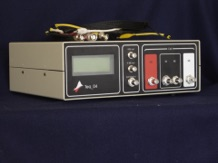
\includegraphics[width=0.5\textwidth]{Figures/Figura_potenciostato}
  \caption{Potentiostat used for electrochemical characterization.}
  \label{fig:Figura_potenciostato}
\end{figure}

\section{Functional Printed Electronics}
Taking advantage of technological advances in micro and nano electronics, it was decided to implement the biosensors using printing techniques, seeking in this way to have disposable sensor arrays, of simple manufacturing and high production scale. The biosensors can be printed on ceramic (Al\textsubscript{2}O\textsubscript{3}), acrylic or PMMA (Methyl Methacrylate Polymer) substrates, or on flexible material like PET (Polyethylene Terephthalate), Valox, etc., using different techniques, such as Screen Printing or Inkjet printing.

Silk-screen printing, typical of thick film technology, allows the manufacture of electronic circuits and sensors that are obtained by depositing layers of inks (typically resistive, conductive and dielectric), by means of a rubber spatula that moves transversely through a mesh or mask, with a given pattern, on an isolated substrate, usually ceramic. The spatula forces the ink to pass through the openings of the stainless steel mesh. They are subsequently sintered at peak temperatures of 850ºC to remove the solvents from the inks, fix the electrical characteristics of the inks and adhere the layers to the substrate (Figure ~\ref{fig:Figura_serigrafia}).

\begin{figure}[H]
  \centering
    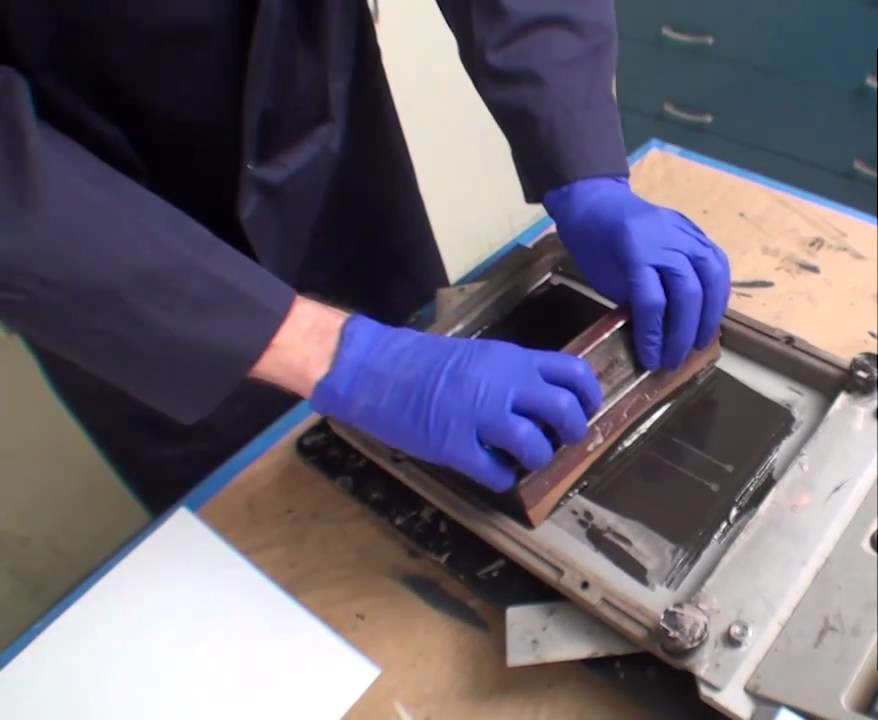
\includegraphics[width=0.5\textwidth]{Figures/Figura_serigrafia}
  \caption{Manual Silk-screen printing.}
  \label{fig:Figura_serigrafia}
\end{figure}

Inkjet printing uses piezoelectric heads to deposit ink droplets according to software controlled coordinates. The inks can be conductive, semiconductive, or dielectric (Figure ~\ref{fig:Figura_inkjet_dimatix}).

\begin{figure}[H]
  \centering
    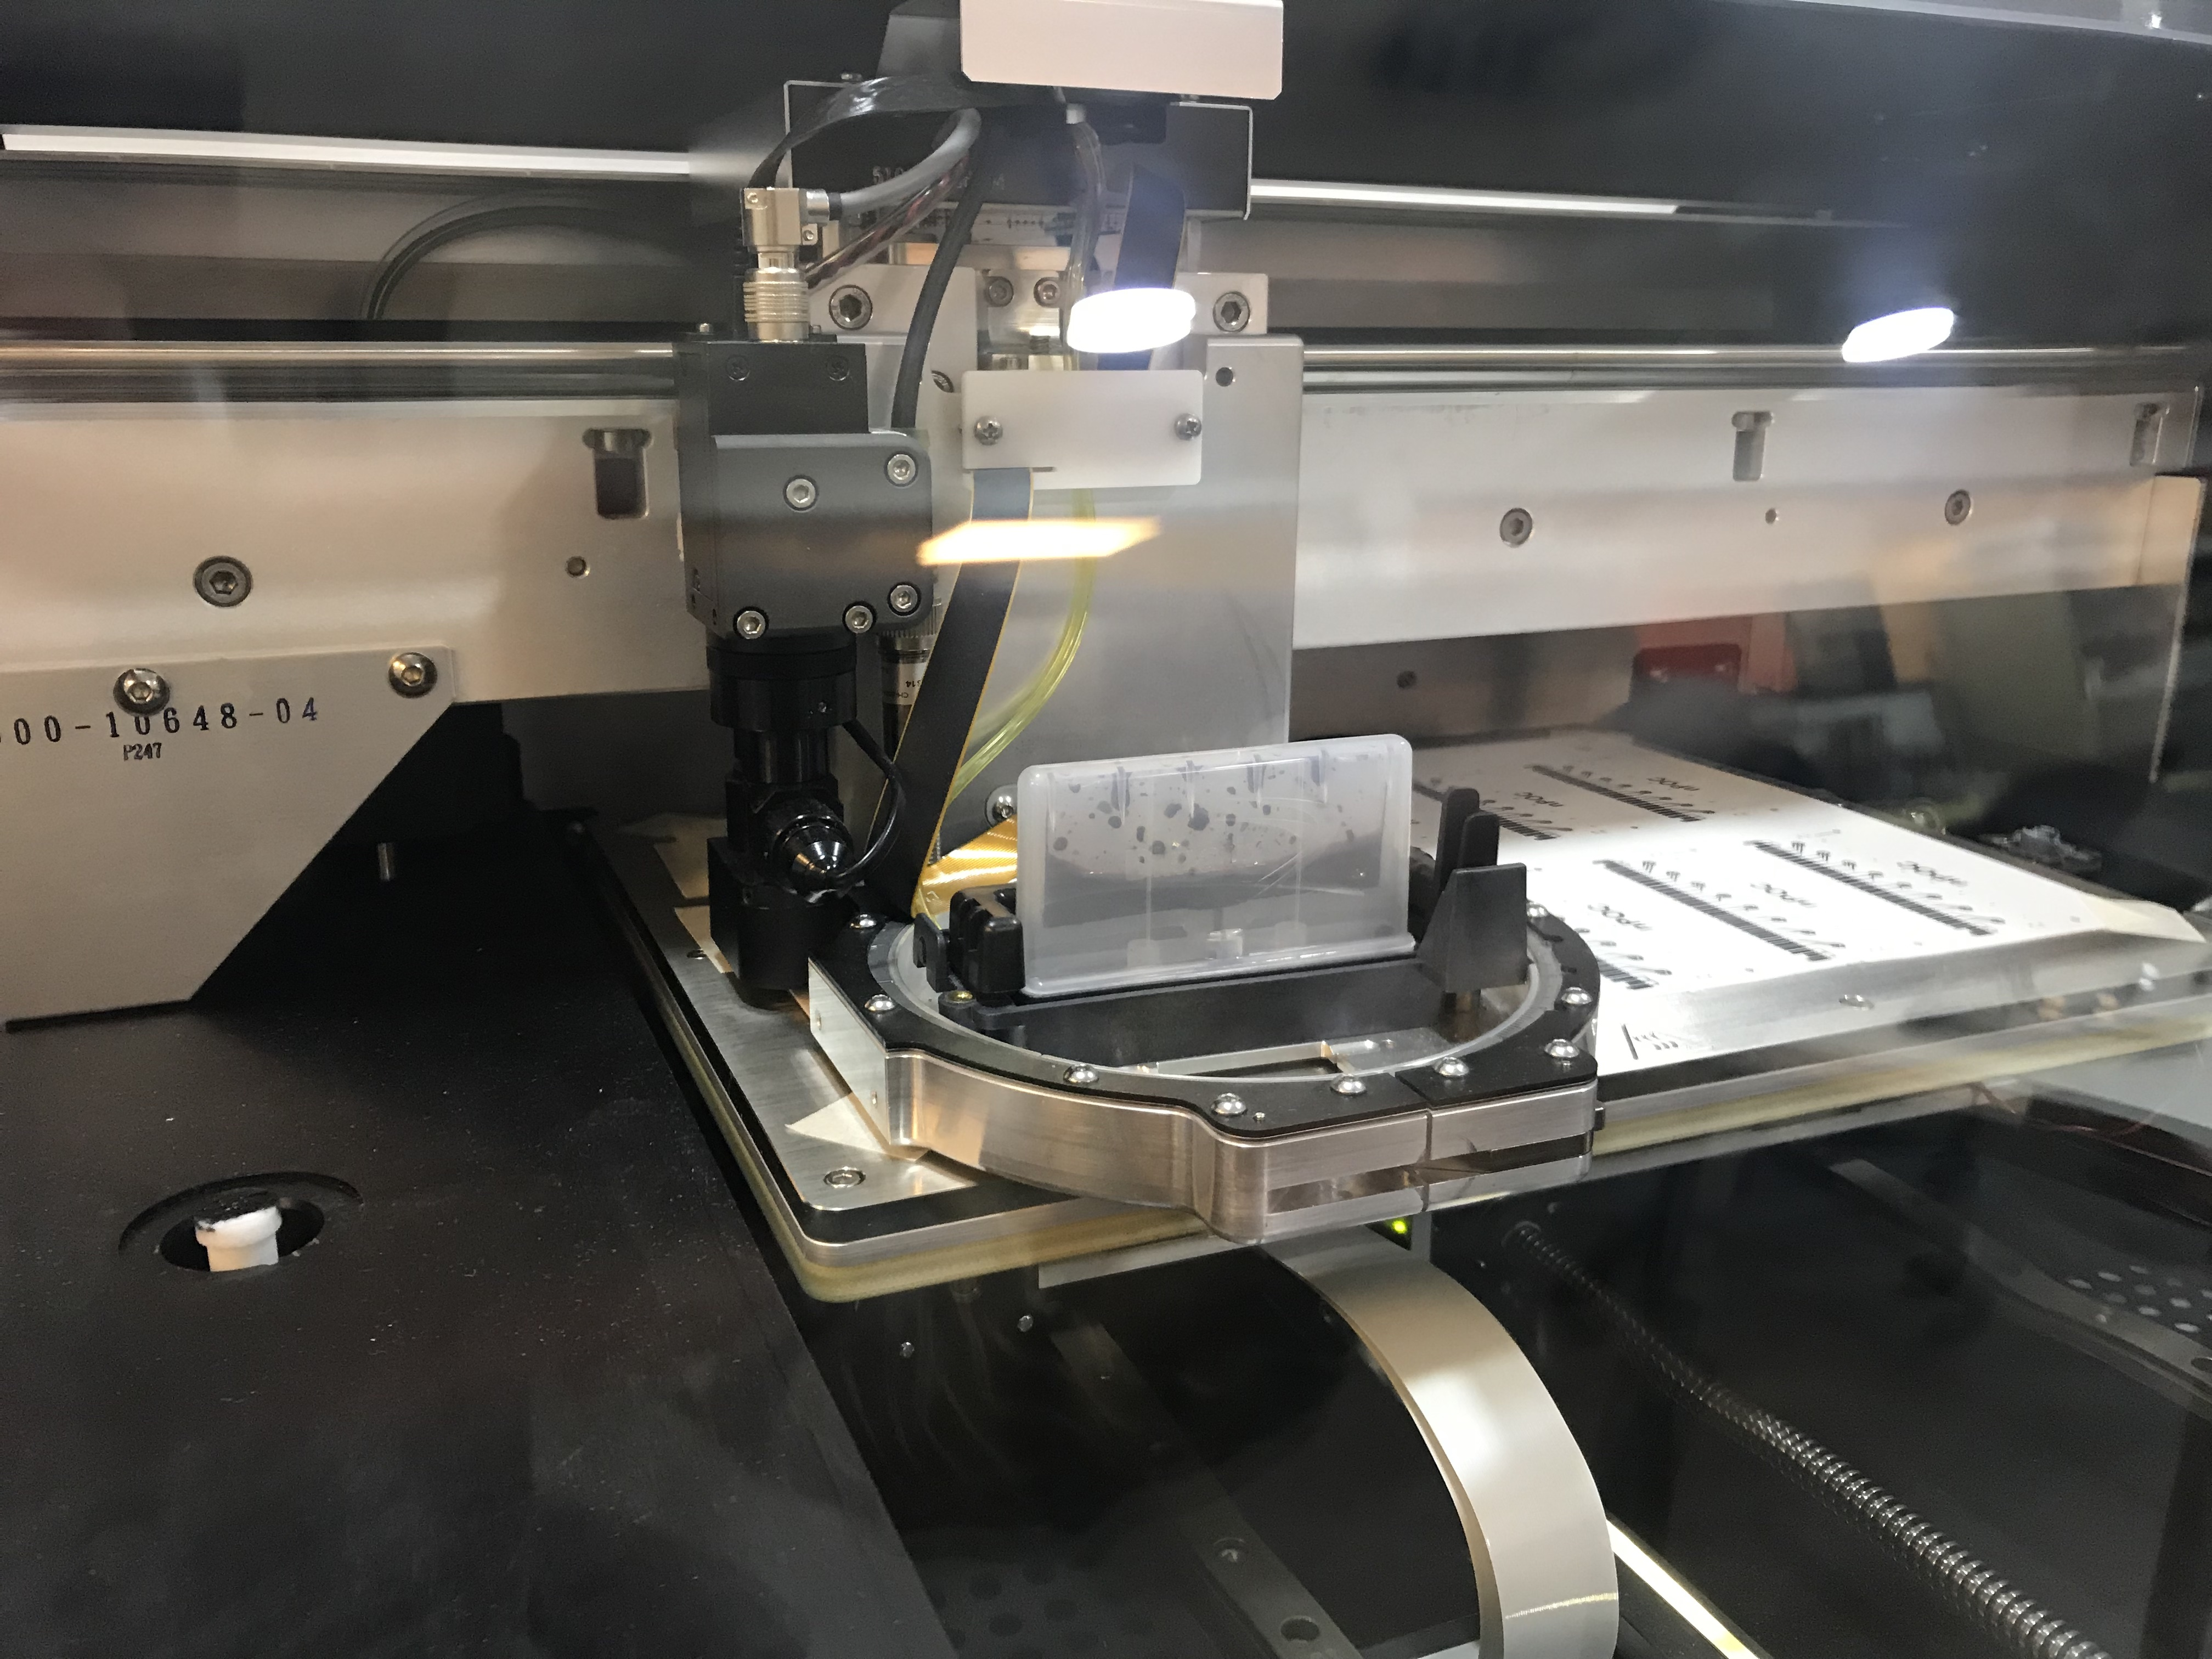
\includegraphics[width=0.5\textwidth]{Figures/Figura_inkjet_dimatix}
  \caption{Inkjet printing.}
  \label{fig:Figura_inkjet_dimatix}
\end{figure}

In this thesis, an electrochemical biosensor on flexible substrate is implemented using an Inkjet printer and the amperometric method is used to characterize it. The versatility, ease of use and innovative type of manufacturing are some of the most notable reasons why it was decided to carry out the present project in an inkjet printer.

\subsection{Inkjet printer}
As mentioned, the Inkjet type printer uses a piezoelectric head for ink deposition  (Figure ~\ref{fig:Figura_Piezoelectrico}). This head contains a reservoir with a crystal that, when a potential is applied, it moves generating a mechanical force in the tank, which causes the ejection of a drop of ink.

\begin{figure}[H]
  \centering
    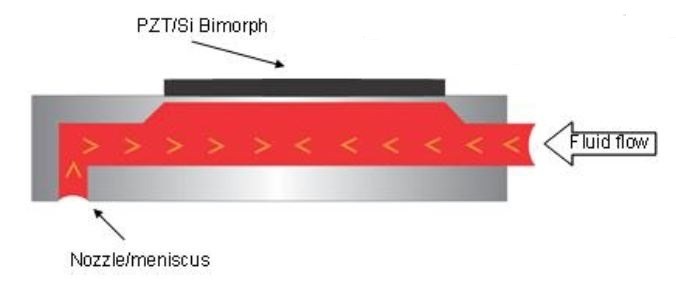
\includegraphics[width=0.5\textwidth]{Figures/Figura_Piezoelectrico}
  \caption{Piezoelectric head diagram.}
  \label{fig:Figura_Piezoelectrico}
\end{figure}

For this, a waveform specified by the manufacturer must be applied (Figure ~\ref{fig:Figura_Waveform_Dimatix}), although it must be modified for each type of ink.

\begin{figure}[H]
  \centering
    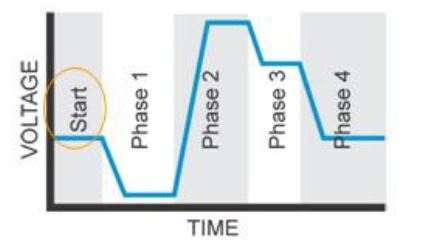
\includegraphics[width=0.5\textwidth]{Figures/Figura_Waveform_Dimatix}
  \caption{Waveform specified for piezoelectric print head.}
  \label{fig:Figura_Waveform_Dimatix}
\end{figure}

In the stage called $``$Start$"$ or also identified as $``$Standby$"$, the piezoelectric is slightly deflected generating an ink meniscus, preventing the involuntary ink drop. In $``$phase 1$"$ the electric potential is decreased and the piezoelectric moves upwards, allowing the reservoir to fill. In $``$phase 2$"$ the voltage increases, initiating the formation of the drop. Once the drop is formed, in $``$phase 3$"$ the voltage decreases again, releasing the drop from the head. $``$Phase 4$"$ is the return to the $``$Start$"$ electric potential (Figure ~\ref{fig:Figura_etapas_eyector}).

\begin{figure}[H]
  \centering
    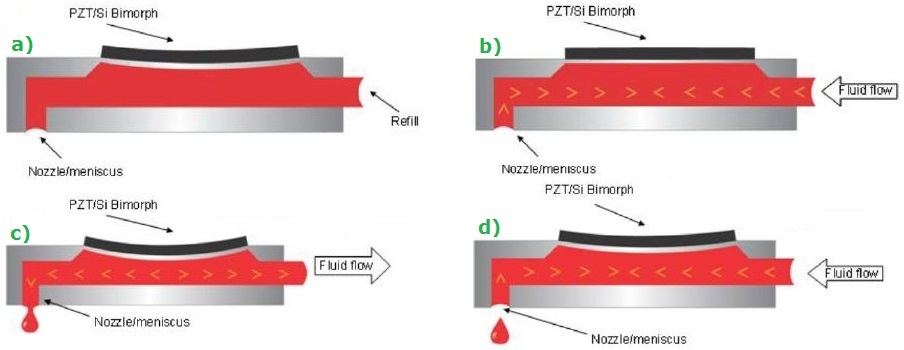
\includegraphics[width=0.8\textwidth]{Figures/Figura_etapas_eyector}
  \caption{a) Start/Standby Stage, b) Phase 1, c) Phase 2, d) Phase 3 and back to Standby.}
  \label{fig:Figura_etapas_eyector}
\end{figure}

The modifiable parameters of this waveform are the voltage level (percentage relative to the voltage set to the ejector), the slew rate that specifies the slope of the ramps between phases and the duration of each segment \cite{DimatixUM}.

The head, responsible for ejecting the ink, is a piece of \textit{MEMS} type (Micro-Electro-Mechanical Systems). Because of this, they are about the size of a thermal inkjet printer, but superior in technology (Figure ~\ref{fig:Figura_cabezal}).

\begin{figure}[H]
  \centering
    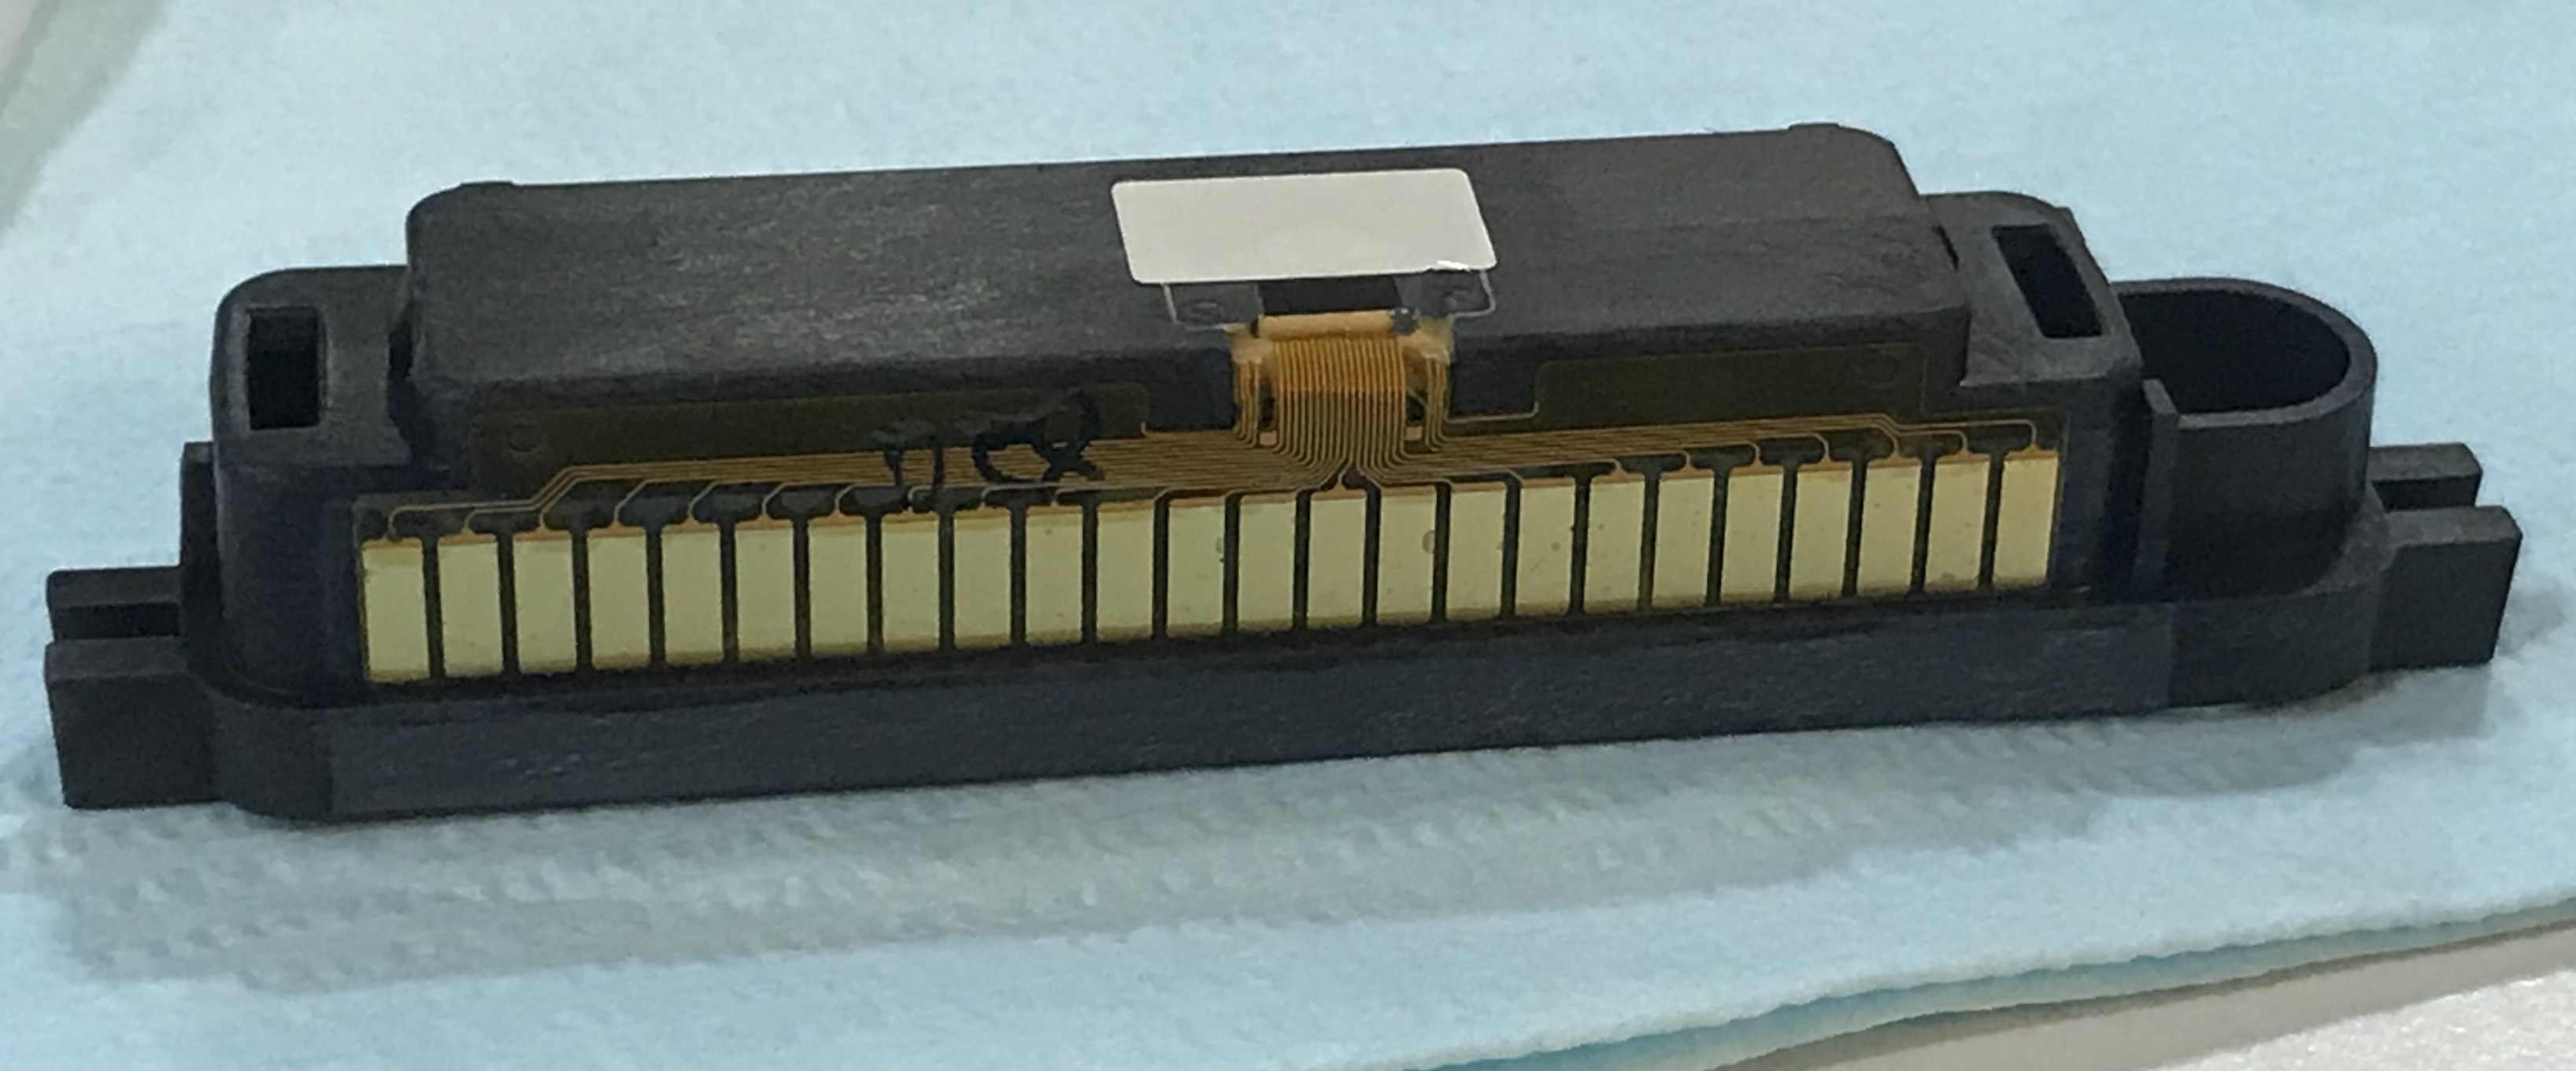
\includegraphics[width=0.5\textwidth]{Figures/Figura_cabezal}
  \caption{Fujifilm Dimatix DMP-2850 Printer Head.}
  \label{fig:Figura_cabezal}
\end{figure}

The one corresponding to the Fujifilm Dimatix DMP2850 printer has 16 ejectors, with which different combinations can be made, achieving different spacing between drops and therefore, different line widths. The complete cartridge consists of the head and a 3 ml reservoir, which can be filled with inks of different materials (Figure ~\ref{fig:Figura_cartucho_completo}).

\begin{figure}[H]
  \centering
    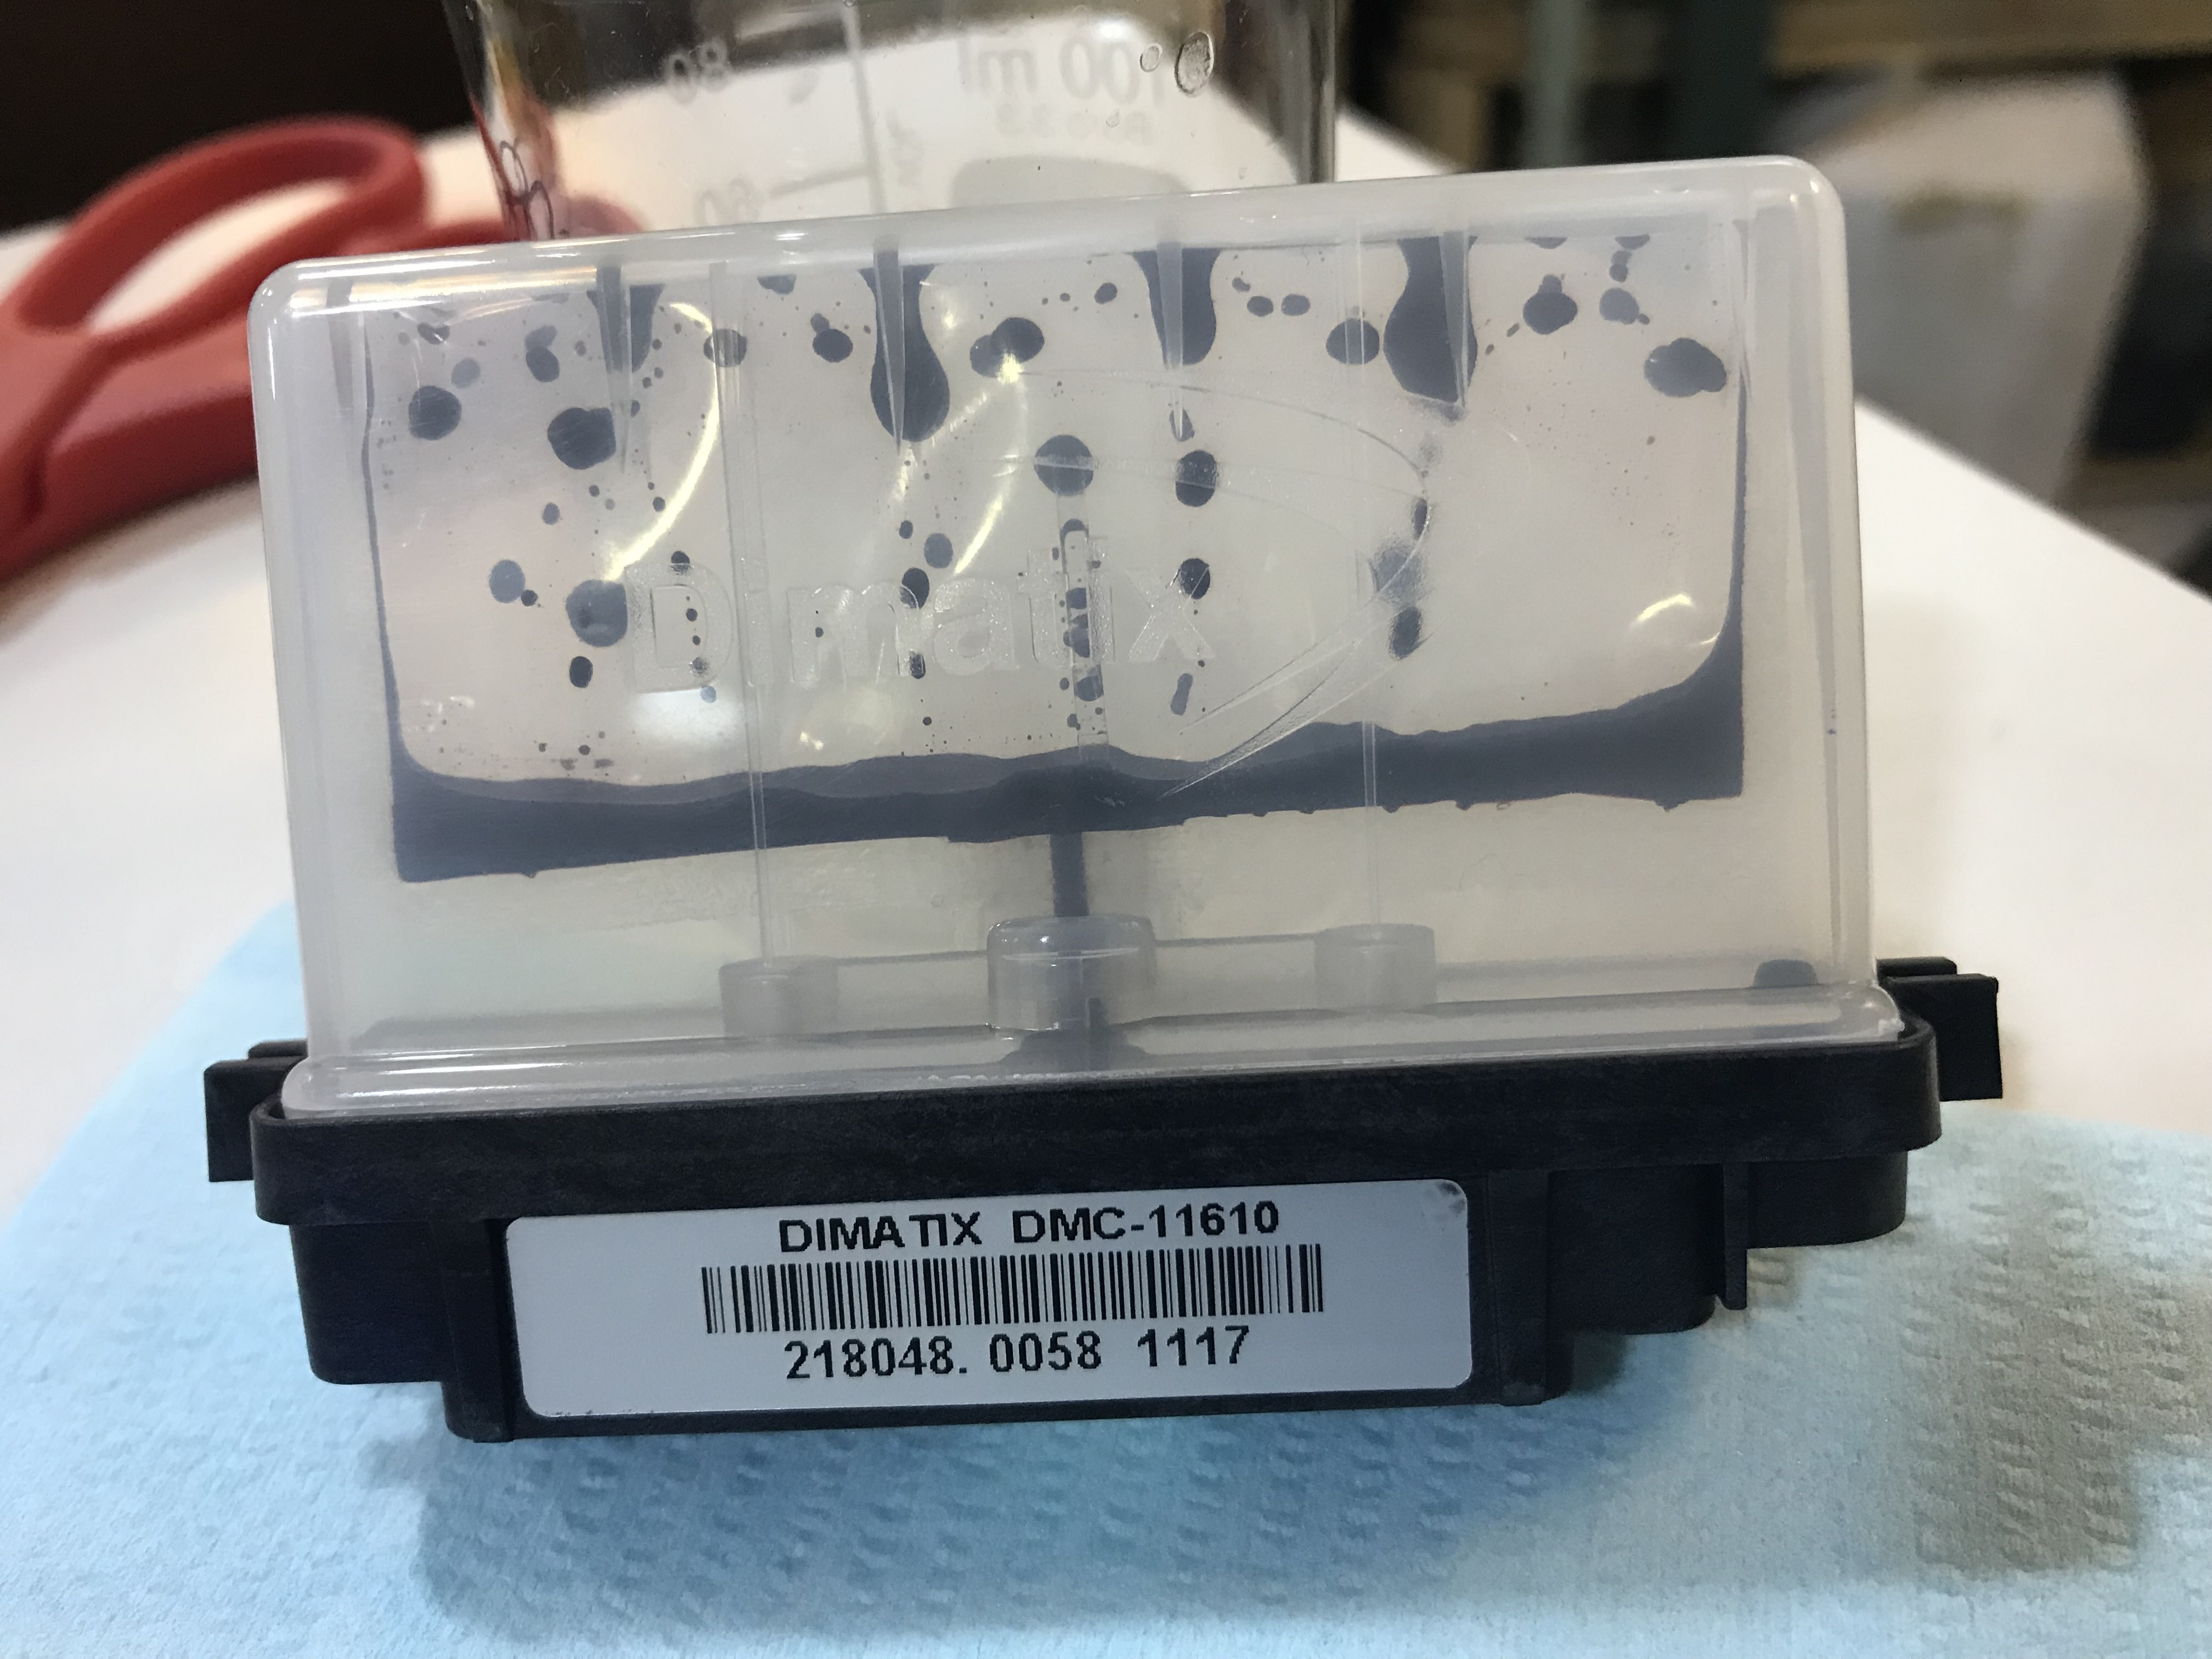
\includegraphics[width=0.5\textwidth]{Figures/Figura_cartucho_completo}
  \caption{Fujifilm Dimatix DMP-2850 Printer Cartridge.}
  \label{fig:Figura_cartucho_completo}
\end{figure}

As examples, Fujifilm reports that graphics, electronics, displays, chemicals, optical objects, photovoltaic objects, 3D mechanical objects, and life science elements such as DNA strands can be printed.

\subsection{Gold nanoparticles ink}
An ink with gold nanoparticles, manufactured by \textit{C-INK} Company under the trade name \textit{Drycure Au-JB 1010B}, will be used in this project  \cite{DrycureAu}. This ink contains nanometric particles of gold (Au). Although the effect of these on the human body has not been proven, extreme caution should be exercised when handling it. For this reason, the manufacturer recommends using it in a good ventilated environment or with an extraction system, using respiratory protection in case of evaporation. Gloves, glasses and work clothes should be worn at all times, especially when handling the ink.

Within its composition there is, given as a percentage in weight, 9-11 \% of Gold, 36-40 \% of water, 48-52 \% of Glycerol, 0.1-1.0 \% of Alcohol, 0.1-0.5 \% of \textit{Acetylene glycol} and 0.1-2.0 \% of Polyester resin.

As physical and chemical characteristics, it is indicated that the ink is liquid, it is a miscible solution, it has a density of 1.10 to 1.20 g/ml and a viscosity of 9 to 11 mPa$\cdot$s.

Since the ink is formulated based on water, it must be kept at low temperatures and hermetically sealed to avoid solvent evaporation or excessive humidity, which can cause alterations in its characteristics (Figure ~\ref{fig:Figura_tinta_Au}).

\begin{figure}[H]
  \centering
    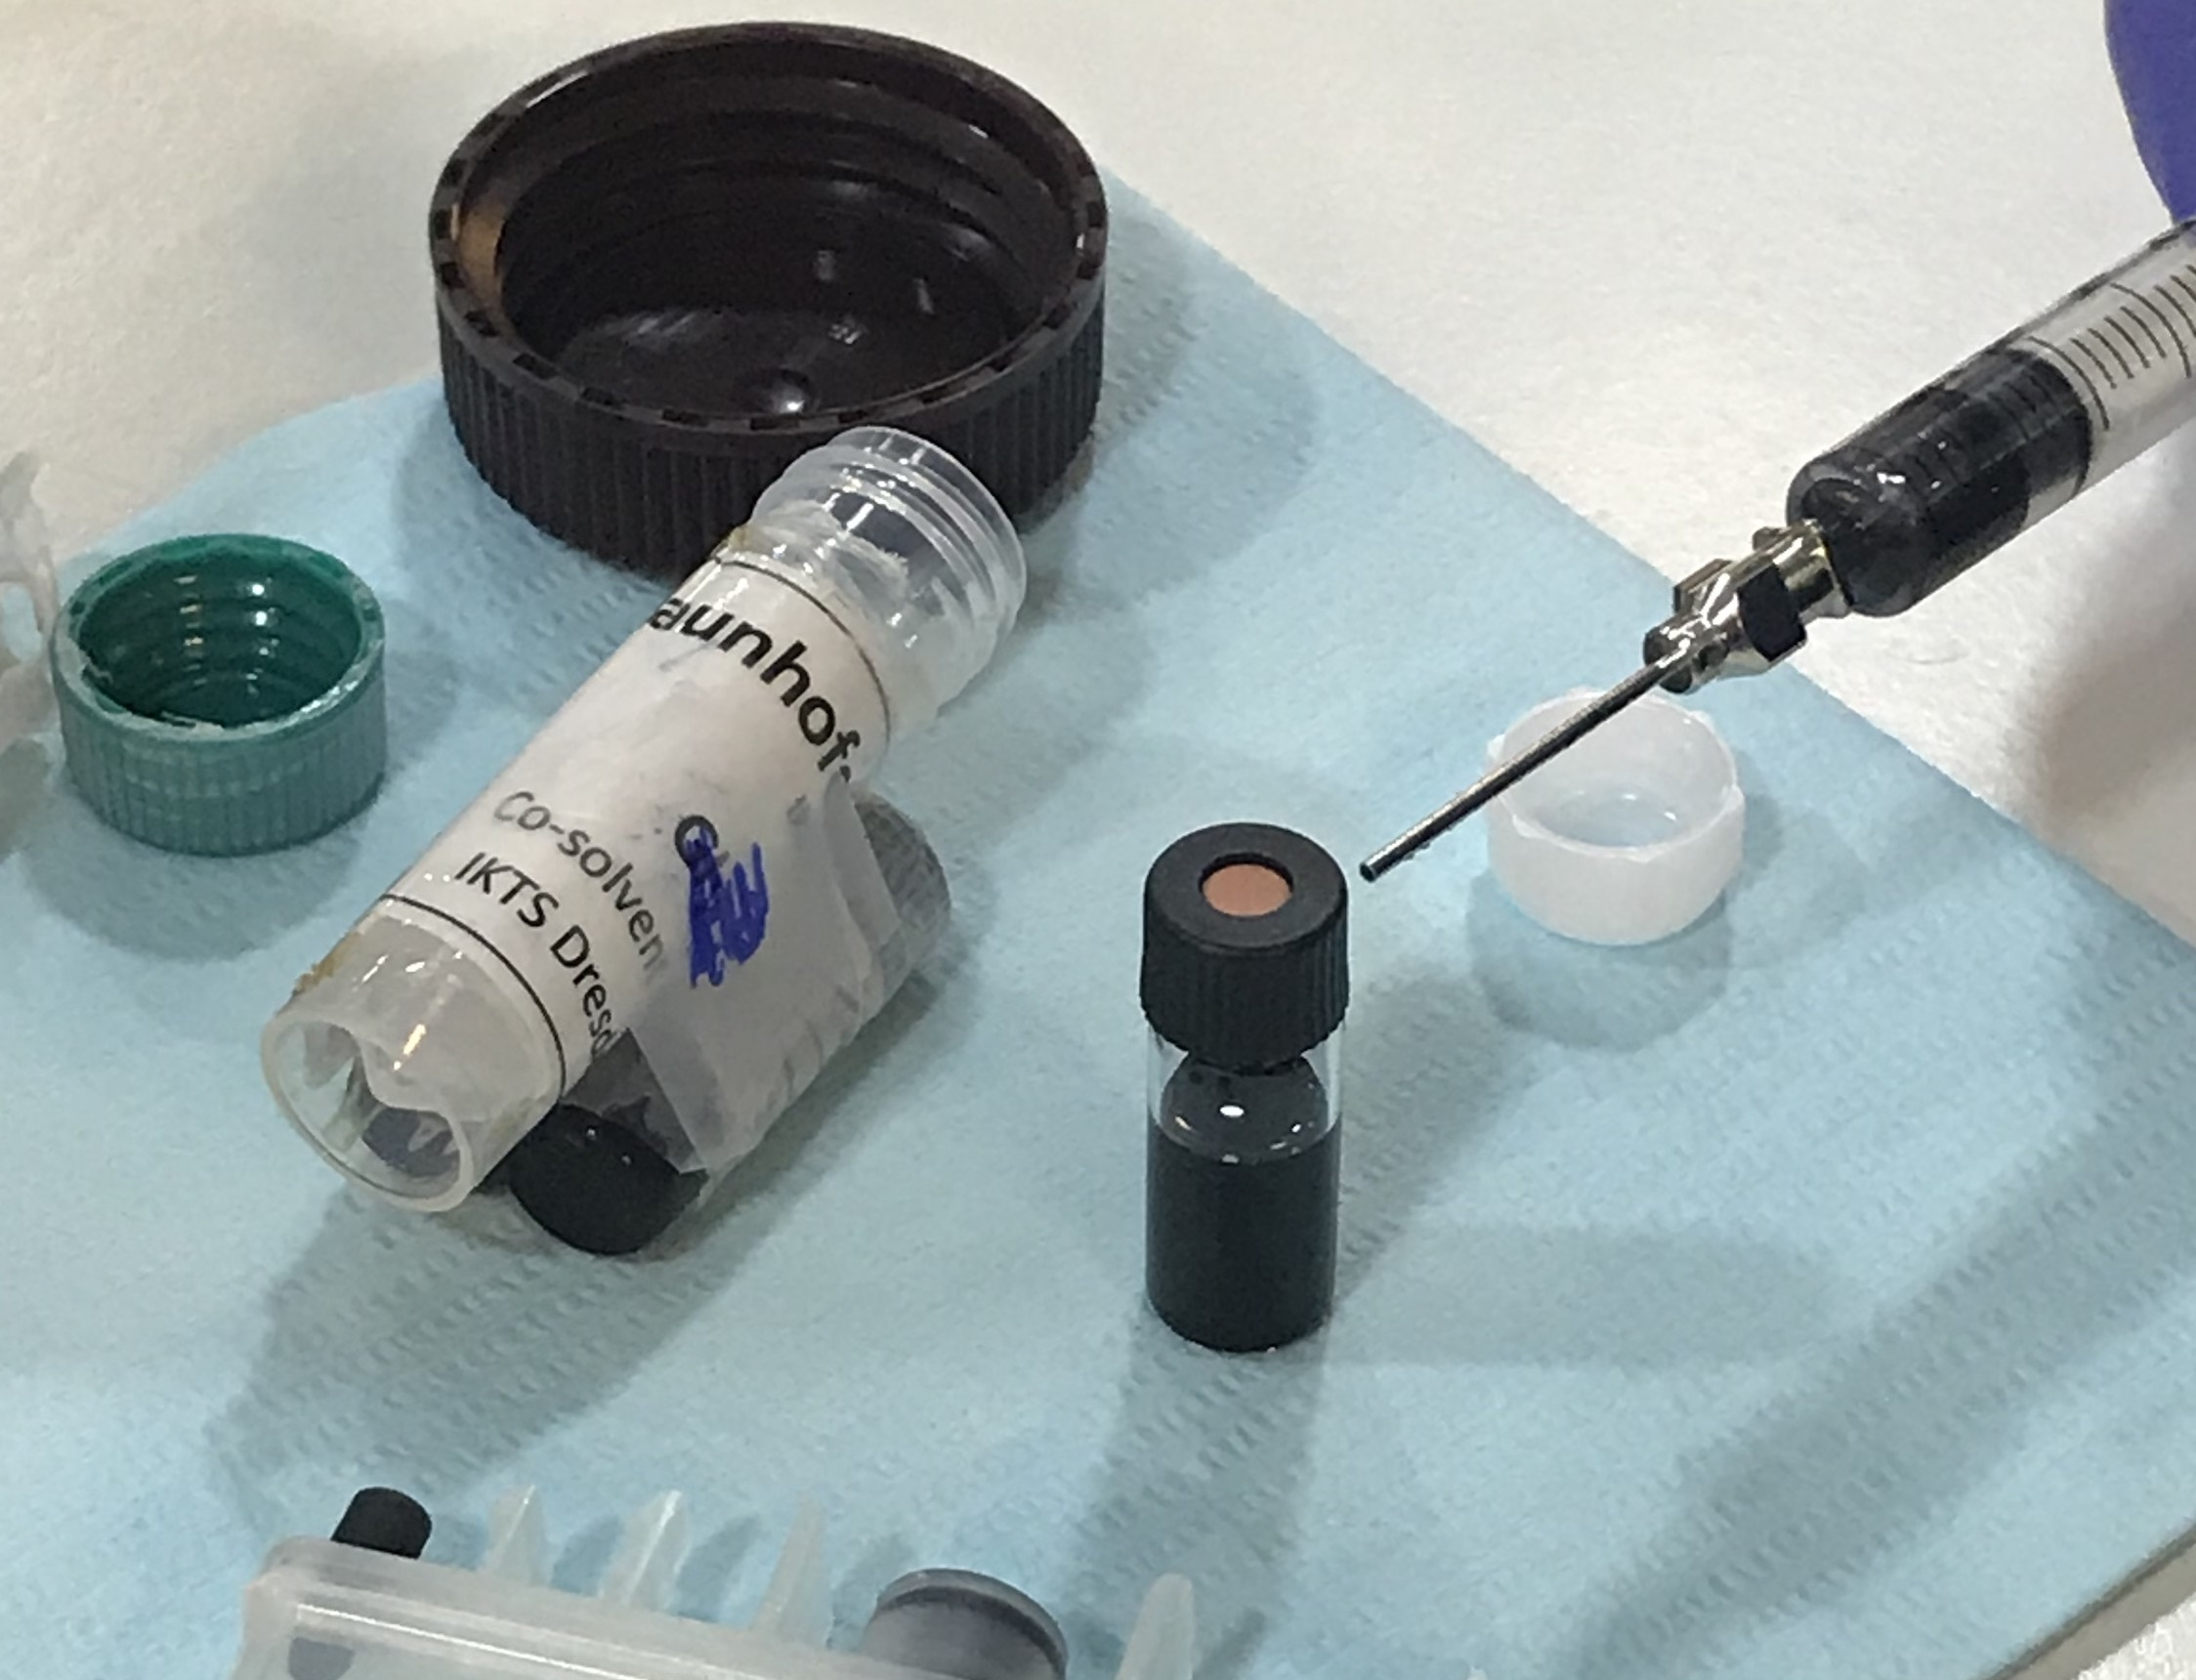
\includegraphics[width=0.5\textwidth]{Figures/Figura_tinta_Au}
  \caption{Hermetically sealed container with gold nanoparticle ink.}
  \label{fig:Figura_tinta_Au}
\end{figure}

\subsection{Photo-definable dielectric ink SU-8}
The dielectric ink used in this project is \emph{PriElex SU-8 2007} from \emph{MicroChem}. It is based on the SU-8 compound, is compatible with Inkjet printing processes and can be thermally cured without the need for UV exposure. (Figure ~\ref{fig:Figura_tinta_SU8}).

Some of its most outstanding advantages are its low curing temperature ($<$ 150ºC), excellent thermal stability and high chemical resistance.

It has a surface tension of 30 dynes/cm, a density of 1,038 g/cm\textsuperscript{3} and a kinematic viscosity of 9.33 cSt. These properties are reported in the manufacturer's datasheet \cite{PriElexSU8}.

\begin{figure}[H]
  \centering
    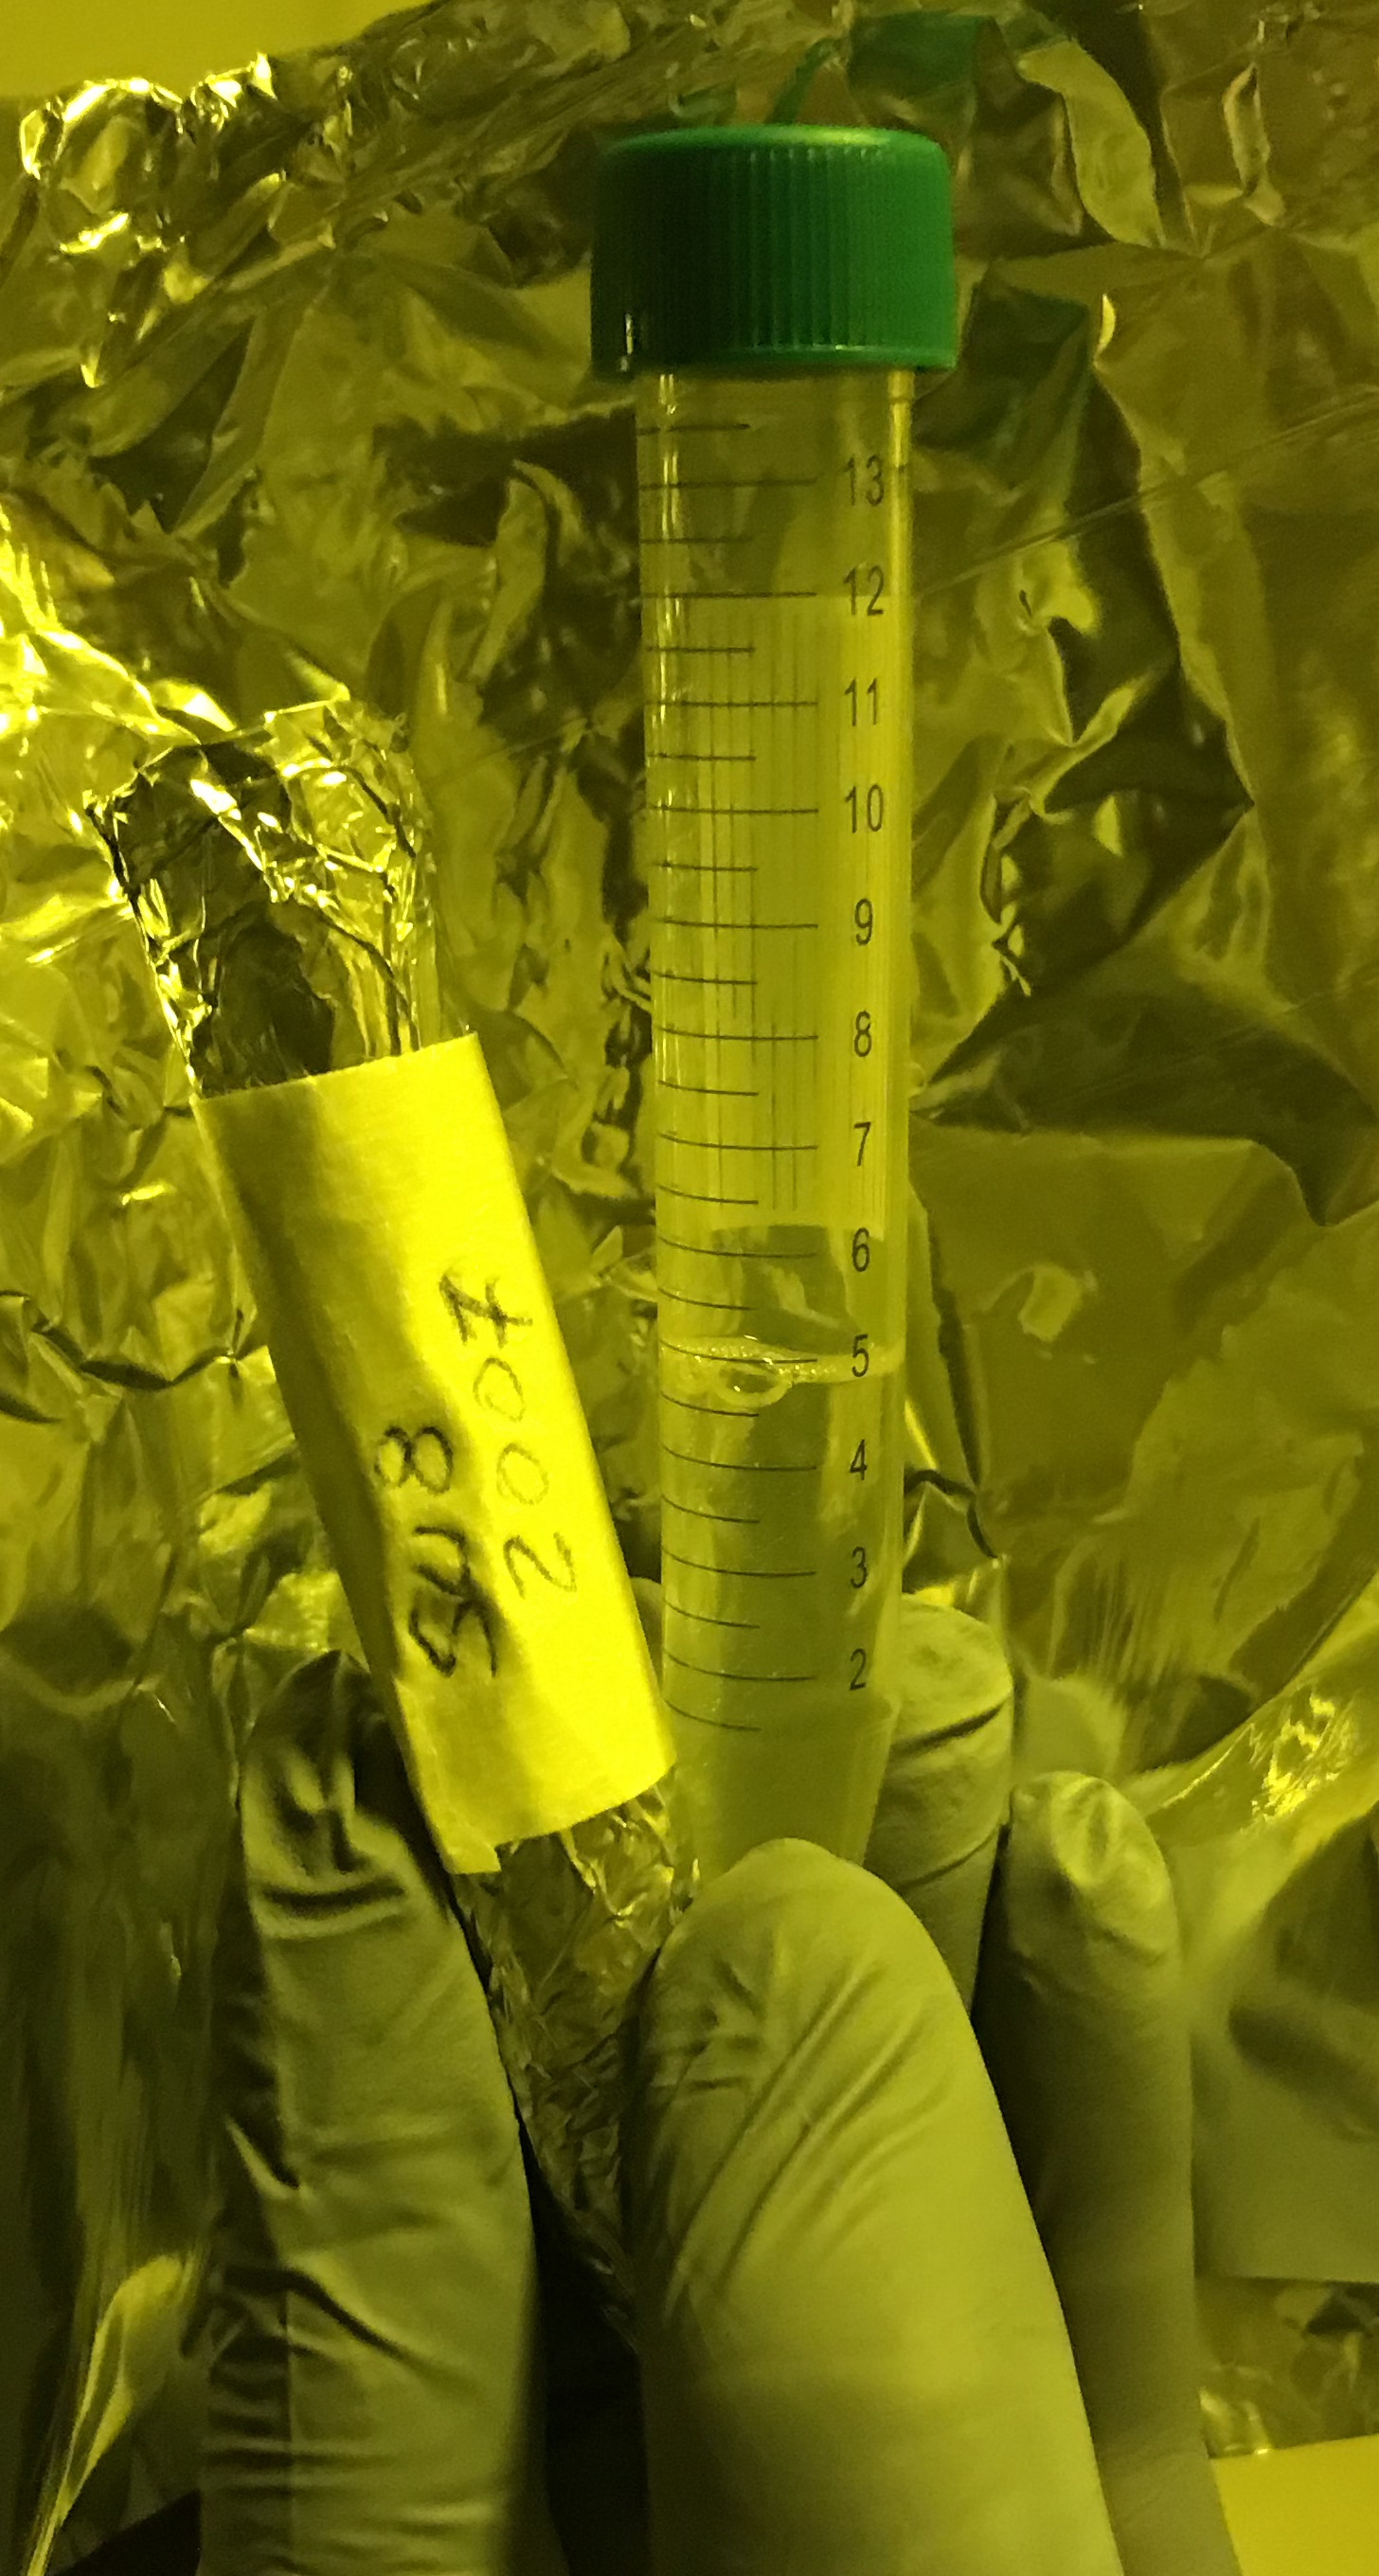
\includegraphics[width=0.2\textwidth]{Figures/Figura_tinta_SU8}
  \caption{SU-8 dielectric ink container.}
  \label{fig:Figura_tinta_SU8}
\end{figure}

\subsection{\textit{Valox} substrate}
The substrate, where the biosensors will be printed, is a film of terephthalite and thermoplastic polybutylene. It is marketed in different thicknesses, for this project the 600 $\mu$m one was used (Figure ~\ref{fig:Figura_Valox}).

This compound has excellent dielectric strength and is easy to handle for thermoforming, stamping, and bending, making it suitable for a wide range of electrical, electronic, and medical applications \cite{Valox}.

\begin{figure}[H]
  \centering
    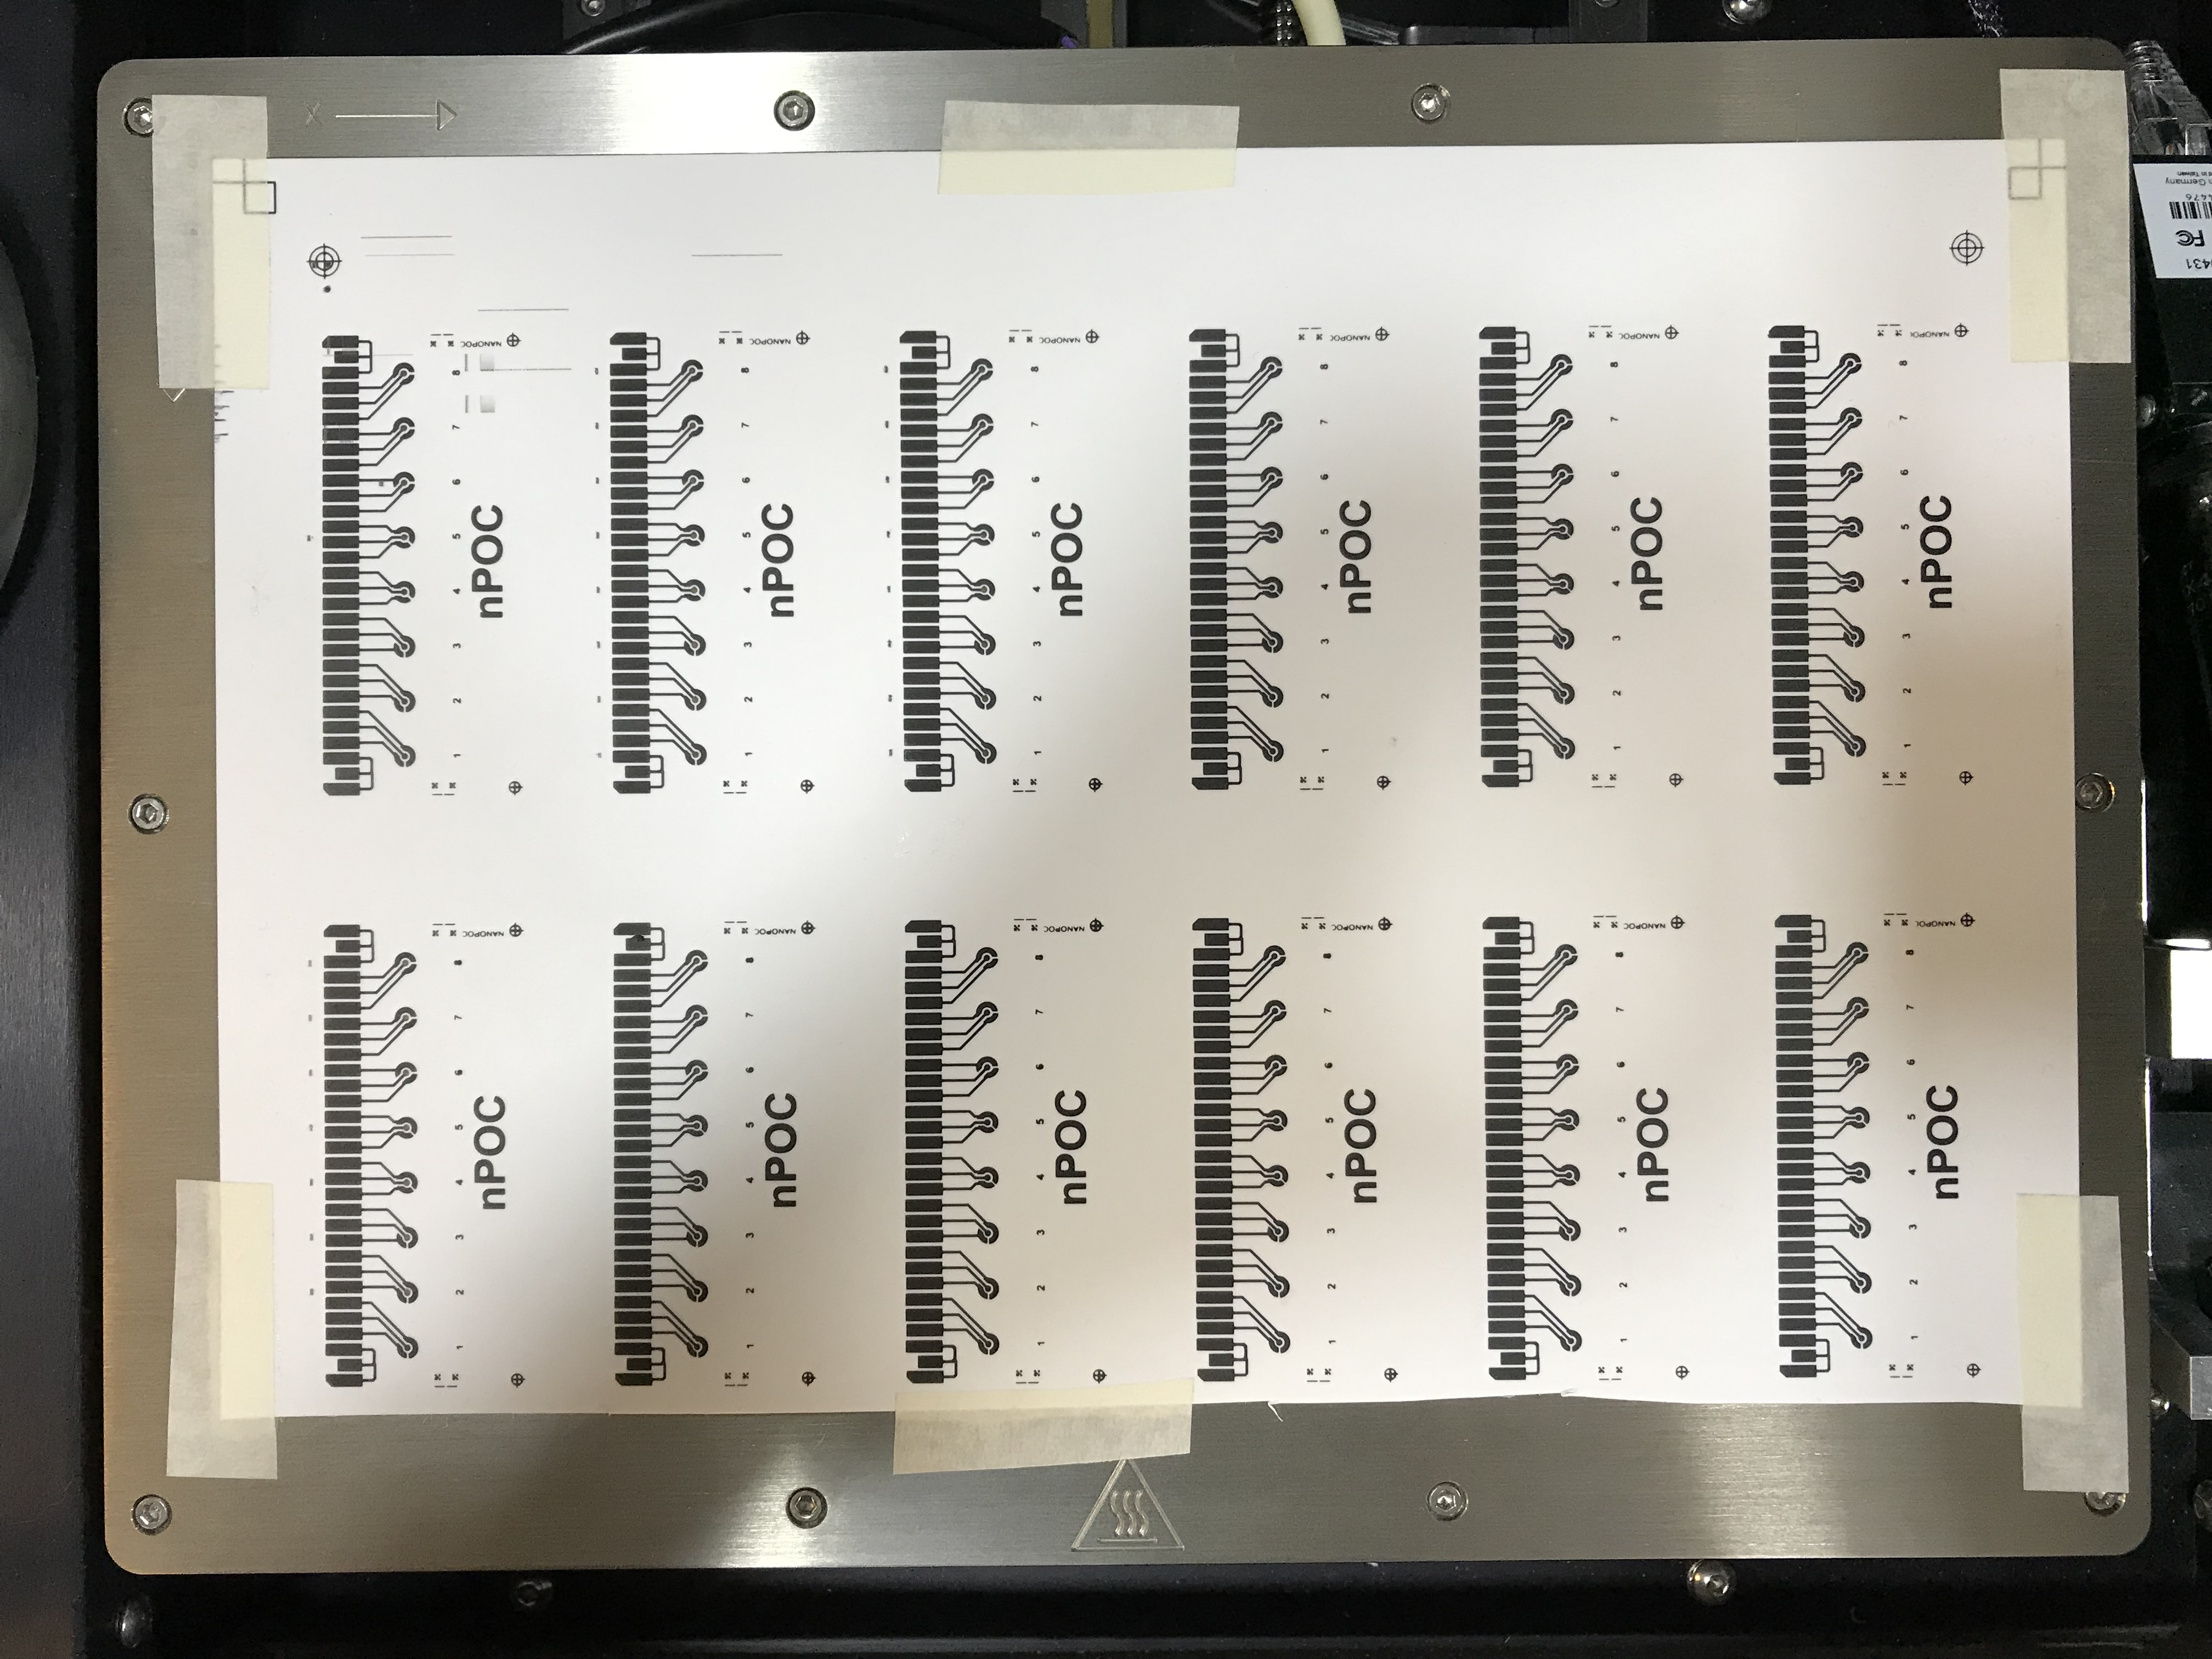
\includegraphics[width=0.55\textwidth]{Figures/Figura_Valox}
  \caption{\textit{Valox} substrate with carbon screen printing.}
  \label{fig:Figura_Valox}
\end{figure}

\section{Characterization techniques}
\subsection{Electrical Characterization}\label{subsec:carac_elec}
Due to the scale at which the nanoparticle ink is printed, it can have microcracks invisible to the eye or low magnification images, however, they are noticeable in microscope magnified images (Figure ~\ref{fig:Figura_Carac_elec}).

\begin{figure}[H]
  \centering
    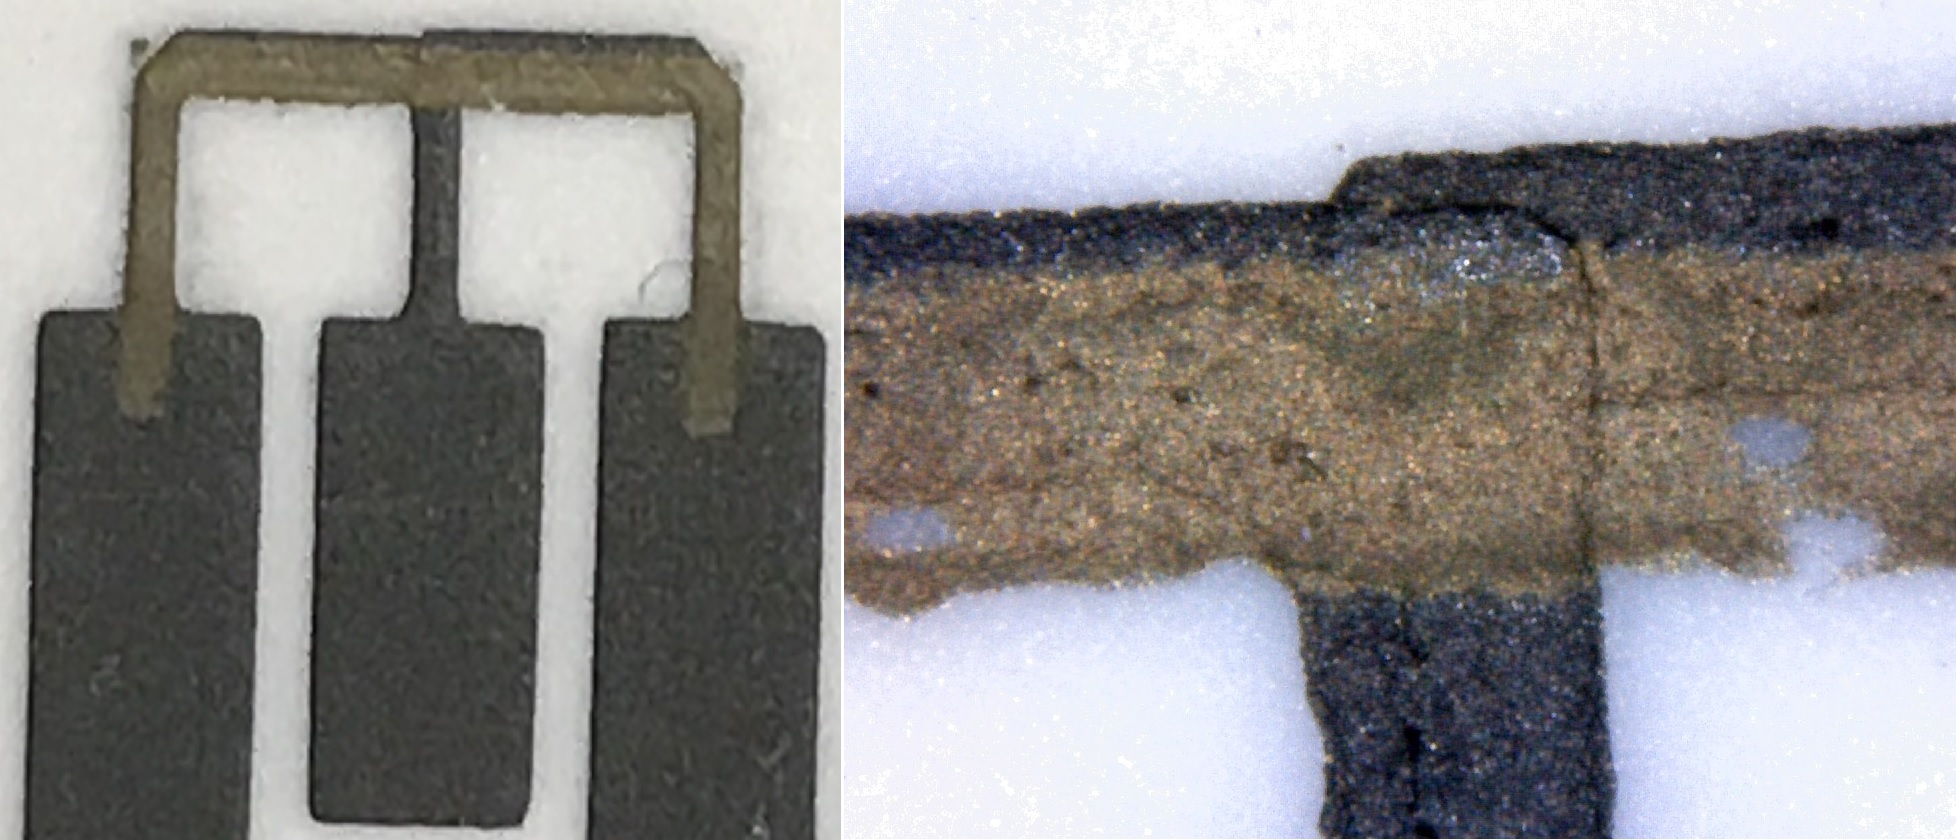
\includegraphics[width=0.5\textwidth]{Figures/Figura_Carac_elec}
  \caption{Image of conventional phone camera (iPhone 7) and image of USB microscope with 1000X Magnification.}
  \label{fig:Figura_Carac_elec}
\end{figure}

Through a 4-point resistance measurement (known as Kelvin method), the physical continuity of the film, the correct operation of the printer and therefore the biosensor working electrode can be ensured.

The method uses two circuits linked by a direct current source. The current from the source flow through one circuit is measured by an ammeter and the other has a voltmeter in parallel with the resistance to be measured. There is also a dual system to the previous one, where there is a verified voltage source with a voltmeter and an ammeter that measures the circulating current through the resistance (Figure ~\ref{fig:Figura_metodo_Kelvin}).

\begin{figure}[H]
  \centering
    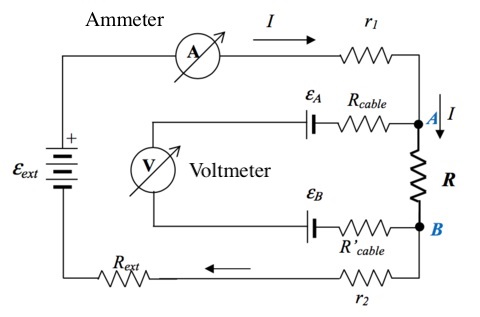
\includegraphics[width=0.5\textwidth]{Figures/Figura_metodo_Kelvin}
  \caption{Four-point measurement circuit.}
  \label{fig:Figura_metodo_Kelvin}
\end{figure}

\subsection{Optical/Dimensional Characterization}
As part of an optical or dimensional characterization it is important to know sizes, thicknesses and roughness.

Sizes can be obtained through the printer's fiducial camera. The software allows measurements of distances between two points and thus obtain all the values required in the characterization (Figure ~\ref{fig:Figura_Cam_Fiducial_Medicion}).

\begin{figure}[H]
  \centering
    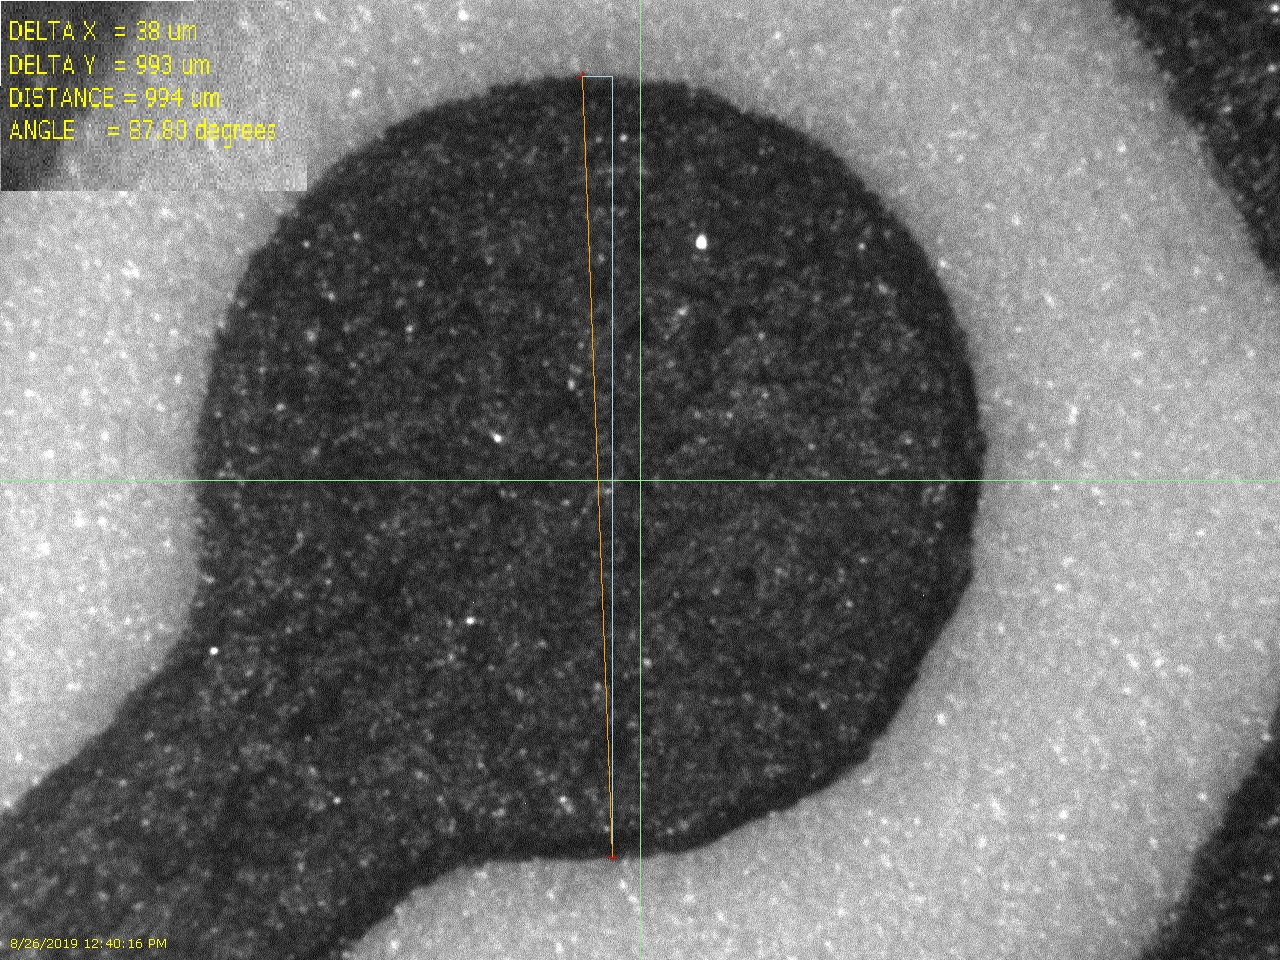
\includegraphics[width=0.5\textwidth]{Figures/Figura_Cam_Fiducial_Medicion}
  \caption{Fiducial camera image with distance measurement.}
  \label{fig:Figura_Cam_Fiducial_Medicion}
\end{figure}

The thickness of the impressions and the roughness of the surfaces can be obtained through a contact profilometer. This equipment, also called a roughness meter, uses a fine tip in contact with the surface to be analyzed (Figure ~\ref{fig:Figura_Stylus}), performing a controlled sweep in a straight line. The height variations detected by this tip are converted into electrical signals and can be recorded or graphed.

\begin{figure}[H]
  \centering
    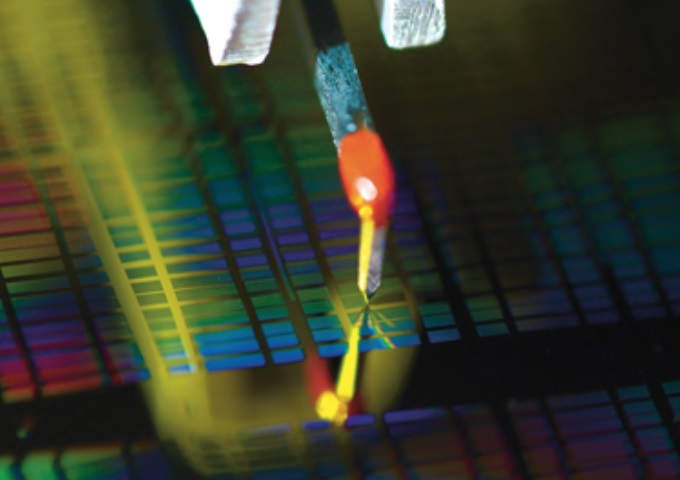
\includegraphics[width=0.5\textwidth]{Figures/Figura_Stylus}
  \caption{Stylus tip image of a contact profilometer.}
  \label{fig:Figura_Stylus}
\end{figure}

Roughness is an important data in characterization, since it defines the working effective area of the biosensor. The smoother the surface, the effective area will approach the geometric area of the electrode.

\subsection{Electrochemical Characterization}
For this work the direct current cyclic voltammetry procedure is used. This electrochemical characterization consists of varying, in a cyclical way, the electrical potential of the working electrode relative to a reference one. Both are immersed in a solution and the resulting current flowing through the working electrode is measured (Figure ~\ref{fig:Figura_circuito_voltametria}). 

\begin{figure}[H]
  \centering
    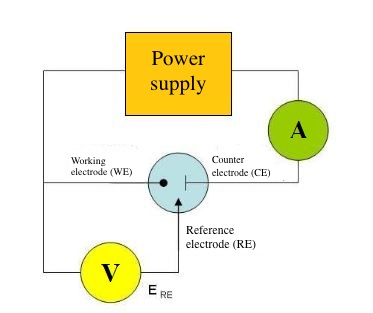
\includegraphics[width=0.65\textwidth]{Figures/Figura_circuito_voltametria}
  \caption{Electrical circuit diagram for direct current cyclic voltammetry.}
  \label{fig:Figura_circuito_voltametria}
\end{figure}

The excitation signal is a linear potential sweep with a triangular wave, which starts from an E1 potential, evolves linearly in time to an E2 potential and then returns to E1 (Figure ~\ref{fig:Figura_Carac_electroquimica}). The speeds of this sweep can range from less than 1 mV/s to hundreds of volts per second \cite{TesisGG}.

\begin{figure}[H]
  \centering
    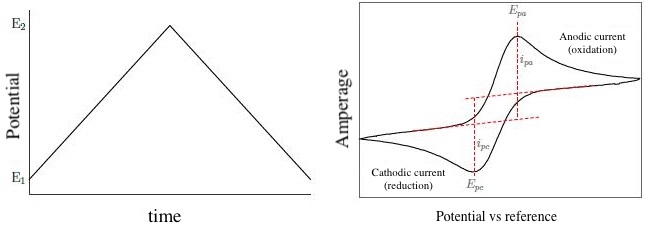
\includegraphics[width=1\textwidth]{Figures/Figura_Carac_electroquimica}
  \caption{Excitation curve and typical voltagram for a reversible redox species. Figure extracted from \cite{TesisGG}.}
  \label{fig:Figura_Carac_electroquimica}
\end{figure}

Ferrocyanide and ferricyanide were used as electrochemical probes. The choice of these probes is due to the reversibility of the \textit{redox} pairs, whose oxidized and reduced species are inexpensive and easy to obtain, soluble in aqueous solution and behave in a quasi-reversible way against electronic exchange.

In the simplest approximation, they are expected to follow the voltammetric behavior described by Randles-Sevcik \ref{ecuacion3}, where the peak current $(i_{p})$ is proportional to the concentration (C), to the square root of the sweep speed (\textit{v}) and to the area (A). The other parameters are considered constant.

\begin{equation}\label{ecuacion3}
i_{p}=0,4463 n F A C \left( \frac{nFvD}{RT} \right) ^{1/2}\
\end{equation}